\documentclass[8pt, handout]{beamer} 

%% Math packages
%%
\usepackage{amsmath,amsthm,amssymb}
% Removes the "Too many math alphabets used in version normal" error.
\newcommand\hmmax{0}
\newcommand\bmmax{0}
\usepackage[new]{old-arrows}
\usepackage{cancel}
\usepackage{mathdots}
\usepackage{venndiagram}
\usepackage{mathrsfs}          % Math script font

% Graphics
%%
\graphicspath{{./}{figs/}}
\usepackage{graphicx}
\usepackage{tikz}
\usetikzlibrary{arrows}
\usetikzlibrary{decorations.markings}
\usetikzlibrary{decorations.pathreplacing}
\usetikzlibrary{patterns}
\usetikzlibrary{shapes.geometric}
\usetikzlibrary{matrix}
\usepackage{tikz-3dplot}
\usepackage{tkz-graph}
\usepackage{tikz-cd}

%% Colors (most are in colors.tex file)
%%
\usepackage{xcolor}
\usepackage{color}
\usepackage{visualalgebra}  %% Put this *after* the TikZ packages
\usepackage{visualalgebraslides}  %% Put this *after* "visualalgebra"

%% Page layout packages
%%
\usepackage{url}
\usepackage{multicol}
\usepackage{multirow}
\usepackage[numbers,square,sort&compress]{natbib}

%% Font and formatting packages
%%
\usepackage[english]{babel}    % Removing this causes compiler error
\usepackage{alltt}             % Like verbatim, but excludes \ and { }
\usepackage{enumerate}         % [shortlabels] option??
\usepackage{comment}
\usepackage{soul}              % strikeout text
\usepackage{bm}                % Bold math
\usepackage[T1]{fontenc}
\usepackage{relsize}

%% Fixes the \mathbf{} not working for fonts under 10pt
\usepackage{cmbright}
\fontencoding{OT1}\fontfamily{cmbr}\selectfont %to load ot1cmbr.fd
\DeclareFontShape{OT1}{cmbr}{bx}{n}{% change bx definition
<->cmbrbx10%
}{}
\normalfont

\makeatletter
\renewcommand*\env@matrix[1][\arraystretch]{%
  \edef\arraystretch{#1}%
  \hskip -\arraycolsep
  \let\@ifnextchar\new@ifnextchar
  \array{*\c@MaxMatrixCols c}}
\makeatother


%%=======================================================================

%% Beamer packages
%%
\mode<presentation>
{
  \usetheme{boadilla} 
  \useinnertheme{rectangles}
  \usecolortheme{dolphin}
}

\setbeamersize{text margin left=6mm}
\setbeamersize{text margin right=6mm}
\setbeamersize{sidebar width right=0mm}
\setbeamersize{sidebar width left=0mm}
\setbeamertemplate{navigation symbols}{}

\def\newblock{\hskip .11em plus .33em minus .07em}

% Other options: ball, circle, square 
\setbeamertemplate{enumerate items}[default]
%\setbeamercolor{enumerate subitem}{fg=red!80!black}
\def\opacity{0.5}
\setbeamercovered{transparent}
%\setbeamercovered{invisible}

\newcommand{\Pause}{}      %% Comment this out => lots more page breaks

\AtBeginSection[]{
  \begin{frame}
  \vfill
  \centering
  \begin{beamercolorbox}[sep=8pt,center,shadow=true,rounded=true]{title}
    \usebeamerfont{title}\insertsectionhead\par%
  \end{beamercolorbox}
  \vfill
  \end{frame}
}

%%====================================================================

\title[Isomorphism theorems!]{Isomorphism theorems!}

\author[\href{mailto:sbagley@westminsteru.edu}{S. Bagley}]
       {\href{mailto:sbagley@westminsteru.edu}{Spencer Bagley}}

\institute[Westminster] { 
  \normalsize With many thanks to Matthew Macauley, \\
  \url{http://www.math.clemson.edu/~macaule/}}

\date[31 Mar 2025]{31 Mar 2025}

\begin{document}

\frame{\titlepage}

%%====================================================================

\begin{frame}{Preview: embeddings vs. quotients} %\Pause

  The difference between \Alert{embeddings} and \Balert{quotient
    maps} can be seen in the subgroup lattice:
  
  \vspace{-2mm}

  %% Subgroups lattices of AGL_1(Z_5), Dic_{10}, and a cave picture
  %%
  \[
  \begin{tikzpicture}[shorten >= -2pt, shorten <= -2pt,scale=.65]
    \tikzstyle{every node}=[font=\small]
    \begin{scope}[shift={(7,1.6)},scale=1.3,yscale=1.2]
      \node(Dic10) at (0,3) {$\Dic_{10}$};
      \node(r) at (-1.5,2) {$C_{10}$};
      \node(s) at (-.5,1.1) {$C_4$}; 
      \node(rs) at (.15,1.1) {$C_4$}; 
      \node(r2s) at (.8,1.1) {$C_4$}; 
      \node(r3s) at (1.45,1.1) {$C_4$};
      \node(r4s) at (2.1,1.1) {$C_4$};
      \node (r5) at (0,0) {$C_2$};
      \node (r2) at (-1.75,1.3) {\color{midgray}$C_5$};
      \node (1) at (0,-1) {\color{midgray}$C_1$};
      \draw (Dic10) to (r); \draw (r) to (r5);
      \draw (Dic10) to (s); \draw (Dic10) to (rs); 
      \draw (Dic10) to (r2s); \draw (Dic10) to (r3s); \draw (Dic10) to (r4s);
      \draw (r5) to (s); \draw (r5) to (rs); \draw (r5) to (r2s);
      \draw (r5) to (r3s); \draw (r5) to (r4s);
      \draw[faded] (1) to (r5); \draw[faded] (1) to (r2); 
      \draw[faded] (r) to (r2); 
    \end{scope}
    %%
    \begin{scope}[shift={(0,0)},scale=1.3,yscale=1.2]
      \node (Fr20) at (0,4) {\color{midgray}$\AGL_1(\Z_5)$};
      \node(s2-t) at (-.15,2.9) {$D_5$};
      \node (t) at (-1.4,2.2) {$C_5$};
      \node (s) at (-.7,2) {\color{midgray}$C_4$};
      \node (st) at (.25,2) {\color{midgray}$C_4$};
      \node (s3t) at (1.15,2) {\color{midgray}$C_4$};
      \node (ts) at (1.8,2) {\color{midgray}$C_4$};
      \node (ts3) at (2.5,2) {\color{midgray}$C_4$};
      \node(s2) at (-.45,1.1) {$C_2$}; 
      \node(ts2) at (.25,1.1) {$C_2$}; 
      \node(sts) at (1.15,1.1) {$C_2$}; 
      \node(s2t2) at (1.8,1.1) {$C_2$};
      \node(s2t) at (2.5,1.1) {$C_2$};
      \node (1) at (0,0) {$C_1$};
      \draw[bend right=5,faded] (Fr20) to (s); 
      \draw[faded] (Fr20) to (st); 
      \draw[faded] (Fr20) to (s3t);
      \draw[faded] (Fr20) to (ts); 
      \draw[faded] (Fr20) to (ts3); 
      \draw[faded] (Fr20) to (s2-t);
      %%
      \draw (s2-t) to (t); \draw (t) to (1);
      \draw (s2-t) to (s2); \draw (s2-t) to (ts2);
      \draw (s2-t) to (sts);
      \draw (s2-t) to (s2t2); 
      \draw[bend left=10] (s2-t) to (s2t);
      %%
      \draw[faded] (s) to (s2); \draw[faded] (st) to (ts2);
      \draw[faded] (s3t) to (sts); \draw[faded] (ts) to (s2t2);
      \draw[faded] (ts3) to (s2t); 
      %%
      \draw (1) to (s2); \draw (1) to (ts2); \draw (1) to (sts);
      \draw (1) to (s2t2); \draw (1) to (s2t);
    \end{scope}
    %%
    \begin{scope}[shift={(13,3)}]
      \node at (0,0) {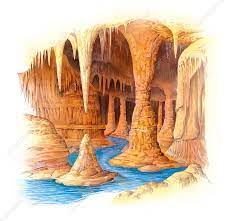
\includegraphics[width=1.4in,height=2in]{cave.jpg}};
    \end{scope}
  \end{tikzpicture}
  \]

  In one of these groups, $D_5$ is a \Alert{subgroup}, and it rises up from the floor.
  
  \bigskip
  In the other, it arises as a \Balert{quotient}, and it descends from the ceiling.

  \bigskip\Pause
  
  This, and much more, will be consequences of the celebrated
  \textbf{isomorphism theorems}.
 
\end{frame}

%%====================================================================

\begin{frame}{Preview: subgroups, quotients, and subquotients} %\Pause

%% Subgroup lattice of the derived series of SL2(Z3), and two short exact sequences
  %%

  Often, we'll see familiar subgroup lattices in the middle of a larger
  lattice. \bigskip

  These are called \textbf{subquotients}.
  
  \[
  \begin{tikzpicture}[shorten >= -2pt, shorten <= -2pt,scale=.55]
    %%
    %\tikzstyle{every node}=[font=\small]
    \tikzstyle{B} = [draw, very thick]
    \begin{scope}[shift={(0,0)},xscale=.75]
      \node (G) at (-.5,8.5) {$\SL_2(\Z_3)$};
      \node (Q8) at (-2.5,6) {$Q_8$};
      \node (C6-1) at (.5,5) {$C_6$};
      \node (C6-2) at (1.6,5) {$C_6$};
      \node (C6-3) at (2.7,5) {$C_6$};
      \node (C6-4) at (3.95,5) {$C_6$};
      \node (C4-1) at (-3.75,4) {$C_4$};
      \node (C4-2) at (-2.5,4) {$C_4$};
      \node (C4-3) at (-1.25,4) {$C_4$};
      \node (C3-1) at (.9,3) {$C_3$};
      \node (C3-2) at (2,3) {$C_3$};
      \node (C3-3) at (3.1,3) {$C_3$};
      \node (C3-4) at (4.35,3) {$C_3$};
      \node (C2) at (-2.5,2) {$C_2$};      
      \node (1) at (-2.5,0) {$C_1$};
      %%
      \draw[f] (1) -- (C2);
      \draw[f] (1) -- (C3-1);
      \draw[f] (1) -- (C3-2);
      \draw[f] (1) -- (C3-3);
      \draw[f] (1) -- (C3-4);
      \draw[B] (C2) -- (C4-1);
      \draw[B] (C2) -- (C4-2);
      \draw[B] (C2) -- (C4-3);
      \draw[f] (C2) -- (C6-1);
      \draw[f] (C2) -- (C6-2);
      \draw[f] (C2) -- (C6-3);
      \draw[f] (C2) -- (C6-4);
      \draw[f] (C3-1) -- (C6-1);
      \draw[f] (C3-2) -- (C6-2);
      \draw[f] (C3-3) -- (C6-3);
      \draw[f] (C3-4) -- (C6-4);
      \draw[B] (C4-1) -- (Q8);
      \draw[B] (C4-2) -- (Q8);
      \draw[B] (C4-3) -- (Q8);
      \draw[f] (G) -- (Q8);
      \draw[f] (G) -- (C6-1);
      \draw[f] (G) -- (C6-2);
      \draw[f] (G) -- (C6-3);
      \draw[f] (G) -- (C6-4);
    \end{scope}
    %%
    \begin{scope}[shift={(8.5,0)},xscale=.75]
      %\tikzstyle{every node}=[font=\small]
      \node at (-.5,1) {\small \emph{subgroup of a quotient}};
      \node (G) at (-.5,8.5) {$A_4$};
      \node (Q8) at (-2.5,6) {$V_4$};
      \node (C6-1) at (.5,5) {$C_3$};
      \node (C6-2) at (1.6,5) {$C_3$};
      \node (C6-3) at (2.7,5) {$C_3$};
      \node (C6-4) at (3.95,5) {$C_3$};
      \node (C4-1) at (-3.75,4) {$C_2$};
      \node (C4-2) at (-2.5,4) {$C_2$};
      \node (C4-3) at (-1.25,4) {$C_2$};
      \node (C2) at (-2.5,2) {$C_1$};      
      %%
      \draw[B] (C2) -- (C4-1);
      \draw[B] (C2) -- (C4-2);
      \draw[B] (C2) -- (C4-3);
      \draw[f] (C2) -- (C6-1);
      \draw[f] (C2) -- (C6-2);
      \draw[f] (C2) -- (C6-3);
      \draw[f] (C2) -- (C6-4);
      \draw[B] (C4-1) -- (Q8);
      \draw[B] (C4-2) -- (Q8);
      \draw[B] (C4-3) -- (Q8);
      \draw[f] (G) -- (Q8);
      \draw[f] (G) -- (C6-1);
      \draw[f] (G) -- (C6-2);
      \draw[f] (G) -- (C6-3);
      \draw[f] (G) -- (C6-4);
    \end{scope}
    %%
    \begin{scope}[shift={(17,0)},xscale=.75]
      \node at (-2.5,7      ) {\small \emph{quotient of a subgroup}};
      \node (Q8) at (-2.5,6) {$Q_8$};
      \node (C4-1) at (-3.75,4) {$C_4$};
      \node (C4-2) at (-2.5,4) {$C_4$};
      \node (C4-3) at (-1.25,4) {$C_4$};
      \node (C2) at (-2.5,2) {$C_2$};      
      \node (1) at (-2.5,0) {$C_1$};
      %%
      \draw[f] (1) -- (C2);
      \draw[B] (C2) -- (C4-1);
      \draw[B] (C2) -- (C4-2);
      \draw[B] (C2) -- (C4-3);
      \draw[B] (C4-1) -- (Q8);
      \draw[B] (C4-2) -- (Q8);
      \draw[B] (C4-3) -- (Q8);
    \end{scope}
  \end{tikzpicture}
  \]
  
  The \emph{isomorphism theorems} relates the structure of a group to that of its quotients and subquotients.
  

\end{frame}

%%====================================================================
\section{The Fundamental Homomorphism Theorem!}

%%====================================================================

\begin{frame}{Every homomorphism image is a quotient} \Pause
  
  The following is one of the central results in group theory.
  
  \smallskip
  
  \begin{block}{Fundamental homomorphism theorem (FHT), or Noether's isomorphism theorem}
    If $\phi\colon G\to H$ is a homomorphism, then $\Image(\phi)\cong
    G/\Ker(\phi)$.
  \end{block}
  
  \medskip\Pause
  
  The FHT says that every homomorphism can be decomposed into two steps: (i)
  quotient out by the kernel, and then (ii) relabel the nodes via
  $\phi$.
  %%
  %% Commutative diagram of FHT
  %%
  \[
  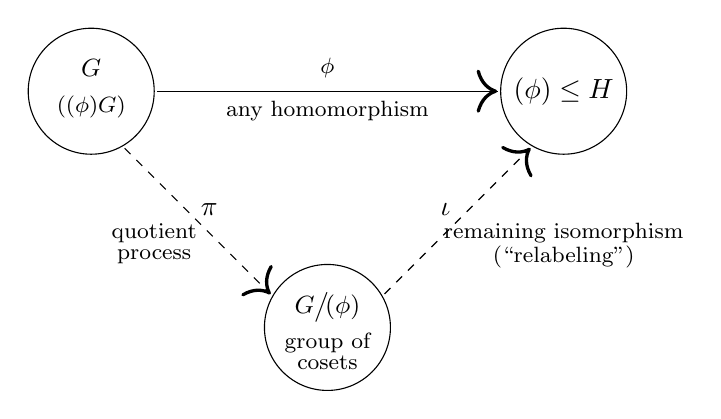
\begin{tikzpicture}[scale=1]
  \tikzset{bigarrow/.style={decoration={markings,mark=at position .99
        with {\arrow[scale=3]{>}}}, postaction={decorate}, 
      shorten >= 1pt, shorten <= 1pt}}
  \tikzstyle{to} = [draw, -stealth]
    \draw (0,0) circle (.8);
    \node at (0,.3) {\small $G$};
    \node at (0,-.2) {\footnotesize ($\Ker(\phi)\normaleq G$)};
    \node at (3,.3) {\footnotesize $\phi$};
    \node at (3,-.25) {\footnotesize any homomorphism};
    %%
    \begin{scope}[shift={(3,-3)}]
      \draw (0,0) circle (.8);
      \node at (0,.25) {\small $G\big/\!\Ker(\phi)$};
      \node at (0,-.2) {\footnotesize group of};
      \node at (0,-.45) {\footnotesize cosets};
    \end{scope}
    %%
    \begin{scope}[shift={(6,0)}]
      \draw (0,0) circle (.8);
      \node at (0,0) {$\Image(\phi)\leq H$};
    \end{scope}
    %%
    \draw [bigarrow] (.8,0) to (5.2,0);
    \draw [bigarrow, dashed] (.4,-.7) to (2.3,-2.6);
    \node at (1.5,-1.5) {$\pi$};
    \node at (.8,-1.8) {\footnotesize quotient};
    \node at (.8,-2.1) {\footnotesize process};
    \draw [bigarrow, dashed] (3.7,-2.6) to (5.6,-.7);
    \node at (4.5,-1.5) {$\iota$};
    \node at (6,-1.8) {\footnotesize remaining isomorphism};
    \node at (6,-2.1) {\footnotesize (``relabeling'')};
  \end{tikzpicture}
  \]
  
\end{frame}

%%====================================================================

\begin{frame}{Visualizing the FHT via Cayley graphs}

  (This is HW 8.14.)

  %%
  %% Commutative diagram of FHT (Cayley graphs)
  %%
  \[
  \begin{tikzpicture}[scale=.9]
   \tikzstyle{every node}=[font=\small]
    \begin{scope}[shift={(0,0)}]
      \draw[cosetBlue, fill=cosetBlue] (45:1) circle (.35);
      \draw[cosetBlue, fill=cosetBlue] (135:1) circle (.35);
      \draw[cosetBlue, fill=cosetBlue] (-45:1) circle (.35);
      \draw[cosetBlue, fill=cosetBlue] (-135:1) circle (.35);
      \draw[cosetBlue, fill=cosetBlue] (45:2) circle (.35);
      \draw[cosetBlue, fill=cosetBlue] (135:2) circle (.35);
      \draw[cosetBlue, fill=cosetBlue] (-45:2) circle (.35);
      \draw[cosetBlue, fill=cosetBlue] (-135:2) circle (.35);
      \draw[cosetBlue, fill=cosetBlue,rotate=45] (1,.35) rectangle (2,-.35);
      \draw[cosetBlue, fill=cosetBlue,rotate=135] (1,.35) rectangle (2,-.35);
      \draw[cosetBlue, fill=cosetBlue,rotate=-45] (1,.35) rectangle (2,-.35);
      \draw[cosetBlue, fill=cosetBlue,rotate=-135] (1,.35) rectangle (2,-.35);
      %%
      \node (1) at (135:2) [v] {$1$};
      \node (i) at (45:2) [v] {$i$};
      \node (k) at (-45:2) [v] {$k$};
      \node (j) at (-135:2) [v] {$j$};
      \node (-1) at (135:1) [v] {$-1$};
      \node (-i) at (45:1) [v] {$-i$};
      \node (-k) at (-45:1) [v] {$-k$};
      \node (-j) at (-135:1) [v] {$-j$};
      \node at (-1.8,.95) {$\mathbf{N}$};
      \node at (-1.8,-.95) {$\mathbf{jN}$};
      \node at (1.8,.95) {$\mathbf{iN}$};
      \node at (1.8,-.95) {$\mathbf{kN}$};
      %%
      \path[b] (1) to (i);
      \path[b] (i) to (-1);
      \path[b] (-1) to (-i);
      \path[b] (-i) to (1);
      %%
      \path[b] (-j) to (-k);
      \path[b] (-k) to (j);
      \path[b] (j) to (k);
      \path[b] (k) to (-j);
      %%
      \path[r] (-k) to (-i);
      \path[r] (-i) to (k);
      \path[r] (k) to (i);
      \path[r] (i) to (-k);
      %% 
      \path[r] (1) to (j);
      \path[r] (j) to (-1);
      \path[r] (-1) to (-j);
      \path[r] (-j) to (1);
      %%
      \path[gg] (1) to (-1);
      \path[gg] (j) to (-j);
      \path[gg] (i) to (-i);
      \path[gg] (k) to (-k);
      %%
      \node at (0,0) {\normalsize $Q_8$};
      \draw[-stealth] (2,0) -- (6.3,0) node[midway,above]{\normalsize $\phi$};
      \draw[-stealth] (0,-2) -- (2,-4) node[midway,below
        left]{\normalsize \quad\small{``\emph{quotient map}''}\quad $\pi$};
    \end{scope}
    %%
    \begin{scope}[shift={(4,-5)}]
    \tikzstyle{every node}=[font=\small]
      \tikzstyle{v} = [circle, draw, fill=lightgray,inner sep=0pt, minimum size=5mm]
      \node at (0,3) {\Large $\phi=\iota\circ\pi$};
      \node (e) at (135:1.5) [v] {$N$};
      \node (h) at (45:1.5) [v] {$iN$};
      \node (v) at (-135:1.5) [v] {$jN$};
      \node (b) at (-45:1.5) [v] {$kN$};
      \draw [bb] (e) to (h);
      \draw [bb] (v) to (b);
      \draw [rr] (e) to (v);
      \draw [rr] (h) to (b);
      \node at (0,0) {\normalsize $Q_8/N$};
      \draw[-stealth] (1.75,1) -- (4,3.5) node[midway,below
        right]{\normalsize $\iota$\quad\small{``\emph{relabeling map}''}};
    \end{scope}
    %%
    \begin{scope}[shift={(8,0)}]
      \tikzstyle{every node}=[font=\small]
      \node (e) at (135:1.5) [v] {$e$};
      \node (h) at (45:1.5) [v] {$v$};
      \node (v) at (-135:1.5) [v] {$h$};
      \node (b) at (-45:1.5) [v] {$r$};
      \draw [bb] (e) to (h);
      \draw [bb] (v) to (b);
      \draw [rr] (e) to (v);
      \draw [rr] (h) to (b);
      \node at (0,0) {\normalsize $V_4$};
    \end{scope}
  \end{tikzpicture}
  \]
  
\end{frame}

%%====================================================================

\begin{frame}{Visualizing the FHT via Cayley tables} 
  
  Here's another way to think about the homomorphism
  \[
  \phi\colon Q_8\longonto V_4,\qquad \phi(i)=v,\;\;\phi(j)=h
  \]
  as the composition of: \smallskip
  \begin{itemize}
  \item a quotient by $N=\Ker(\phi)=\<-1\>=\{\pm1\}$, \smallskip
  \item a \emph{relabeling map} $\iota\colon Q_8/N\to V_4$. 
  \end{itemize}
  
  \vspace{2mm}

  %%
  %% Commutative diagram of FHT: Q_8/<-1>
  %%
  \[
  \begin{tikzpicture}[scale=.42]
  \colorlet{color1}{tLime}
  \colorlet{color-1}{tGreen}
  \colorlet{colori}{tRed}
  \colorlet{color-i}{tPink}
  \colorlet{colorj}{tBlue}
  \colorlet{color-j}{tPurple}
  \colorlet{colork}{tOrange}
  \colorlet{color-k}{tYellow}
  %%  
  \newcommand*{\n}{9}%
    \begin{scope}[shift={(0,0)}]
      \tikzstyle{every node}=[font=\footnotesize]
      %% Left column of colors
      \path[fill=color1] (-.1,8) rectangle ++(1,1);
      \path[fill=color-1] (-.1,7) rectangle ++(1,1);
      \path[fill=colori] (-.1,6) rectangle ++(1,1);
      \path[fill=color-i] (-.1,5) rectangle ++(1,1);
      \path[fill=colorj] (-.1,4) rectangle ++(1,1);
      \path[fill=color-j] (-.1,3) rectangle ++(1,1);
      \path[fill=colork] (-.1,2) rectangle ++(1,1);
      \path[fill=color-k] (-.1,1) rectangle ++(1,1);
      %%
      %% Top row of colors
      \path[fill=color1] (1,9.1) rectangle ++(1,1);
      \path[fill=color-1] (2,9.1) rectangle ++(1,1);
      \path[fill=colori] (3,9.1) rectangle ++(1,1);
      \path[fill=color-i] (4,9.1) rectangle ++(1,1);
      \path[fill=colorj] (5,9.1) rectangle ++(1,1);
      \path[fill=color-j] (6,9.1) rectangle ++(1,1);
      \path[fill=colork] (7,9.1) rectangle ++(1,1);
      \path[fill=color-k] (8,9.1) rectangle ++(1,1);
      %%
      %% All red entries in the table
      \path[fill=color1] (1,8) rectangle ++(1,1);
      \path[fill=color1] (2,7) rectangle ++(1,1);
      \path[fill=color1] (3,5) rectangle ++(1,1);
      \path[fill=color1] (4,6) rectangle ++(1,1);
      \path[fill=color1] (5,3) rectangle ++(1,1);
      \path[fill=color1] (6,4) rectangle ++(1,1);
      \path[fill=color1] (7,1) rectangle ++(1,1);
      \path[fill=color1] (8,2) rectangle ++(1,1);
      %%
      \path[fill=color-1] (1,7) rectangle ++(1,1);
      \path[fill=color-1] (2,8) rectangle ++(1,1);
      \path[fill=color-1] (3,6) rectangle ++(1,1);
      \path[fill=color-1] (4,5) rectangle ++(1,1);
      \path[fill=color-1] (5,4) rectangle ++(1,1);
      \path[fill=color-1] (6,3) rectangle ++(1,1);
      \path[fill=color-1] (7,2) rectangle ++(1,1);
      \path[fill=color-1] (8,1) rectangle ++(1,1);
      %%
      \path[fill=colori] (1,6) rectangle ++(1,1);
      \path[fill=colori] (2,5) rectangle ++(1,1);
      \path[fill=colori] (3,8) rectangle ++(1,1);
      \path[fill=colori] (4,7) rectangle ++(1,1);
      \path[fill=colori] (5,1) rectangle ++(1,1);
      \path[fill=colori] (6,2) rectangle ++(1,1);
      \path[fill=colori] (7,4) rectangle ++(1,1);
      \path[fill=colori] (8,3) rectangle ++(1,1);
      %%
      \path[fill=color-i] (1,5) rectangle ++(1,1);
      \path[fill=color-i] (2,6) rectangle ++(1,1);
      \path[fill=color-i] (3,7) rectangle ++(1,1);
      \path[fill=color-i] (4,8) rectangle ++(1,1);
      \path[fill=color-i] (5,2) rectangle ++(1,1);
      \path[fill=color-i] (6,1) rectangle ++(1,1);
      \path[fill=color-i] (7,3) rectangle ++(1,1);
      \path[fill=color-i] (8,4) rectangle ++(1,1);
      %%
      \path[fill=colorj] (1,4) rectangle ++(1,1);
      \path[fill=colorj] (2,3) rectangle ++(1,1);
      \path[fill=colorj] (3,2) rectangle ++(1,1);
      \path[fill=colorj] (4,1) rectangle ++(1,1);
      \path[fill=colorj] (5,8) rectangle ++(1,1);
      \path[fill=colorj] (6,7) rectangle ++(1,1);
      \path[fill=colorj] (7,5) rectangle ++(1,1);
      \path[fill=colorj] (8,6) rectangle ++(1,1);
      %%
      \path[fill=color-j] (1,3) rectangle ++(1,1);
      \path[fill=color-j] (2,4) rectangle ++(1,1);
      \path[fill=color-j] (3,1) rectangle ++(1,1);
      \path[fill=color-j] (4,2) rectangle ++(1,1);
      \path[fill=color-j] (5,7) rectangle ++(1,1);
      \path[fill=color-j] (6,8) rectangle ++(1,1);
      \path[fill=color-j] (7,6) rectangle ++(1,1);
      \path[fill=color-j] (8,5) rectangle ++(1,1);
      %%
      \path[fill=colork] (1,2) rectangle ++(1,1);
      \path[fill=colork] (2,1) rectangle ++(1,1);
      \path[fill=colork] (3,3) rectangle ++(1,1);
      \path[fill=colork] (4,4) rectangle ++(1,1);
      \path[fill=colork] (5,6) rectangle ++(1,1);
      \path[fill=colork] (6,5) rectangle ++(1,1);
      \path[fill=colork] (7,8) rectangle ++(1,1);
      \path[fill=colork] (8,7) rectangle ++(1,1);
      %%
      \path[fill=color-k] (1,1) rectangle ++(1,1);
      \path[fill=color-k] (2,2) rectangle ++(1,1);
      \path[fill=color-k] (3,4) rectangle ++(1,1);
      \path[fill=color-k] (4,3) rectangle ++(1,1);
      \path[fill=color-k] (5,5) rectangle ++(1,1);
      \path[fill=color-k] (6,6) rectangle ++(1,1);
      \path[fill=color-k] (7,7) rectangle ++(1,1);
      \path[fill=color-k] (8,8) rectangle ++(1,1);
      %%
      \foreach \i in {1,...,\n} {
        \draw [very thin] (\i,1) -- (\i,\n); 
        \draw [very thin] (\i,\n+.1) -- (\i,\n+1.1); 
        \draw [very thin] (1,\i) -- (\n,\i); 
        \draw [very thin] (-.1,\i) -- (.9,\i); 
      } 
      \draw (-.1,1) rectangle ++(1,8);
      \draw (1,9.1) rectangle ++(8,1);
      \node at (0.4,8.5) {$1$};
      \node at (0.4,7.5) {$-1$};
      \node at (0.4,6.5) {$i$};
      \node at (0.4,5.5) {$-i$}; 
      \node at (0.4,4.5) {$j$}; 
      \node at (0.4,3.5) {$-j$};
      \node at (0.4,2.5) {$k$};
      \node at (0.4,1.5) {$-k$};
      %% 
      \node at (1.5,9.6) {$1$};
      \node at (2.5,9.6) {$-1$};
      \node at (3.5,9.6) {$i$};
      \node at (4.5,9.6) {$-i$}; 
      \node at (5.5,9.6) {$j$}; 
      \node at (6.5,9.6) {$-j$};
      \node at (7.5,9.6) {$k$};
      \node at (8.5,9.6) {$-k$};
      %%
      \node at (1.5,8.5) {$1$};
      \node at (1.5,7.5) {$-1$};
      \node at (1.5,6.5) {$i$};
      \node at (1.5,5.5) {$-i$}; 
      \node at (1.5,4.5) {$j$}; 
      \node at (1.5,3.5) {$-j$};
      \node at (1.5,2.5) {$k$};
      \node at (1.5,1.5) {$-k$};
      %%
      \node at (2.5,8.5) {$-1$};
      \node at (2.5,7.5) {$1$};
      \node at (2.5,6.5) {$-i$};
      \node at (2.5,5.5) {$i$}; 
      \node at (2.5,4.5) {$-j$}; 
      \node at (2.5,3.5) {$j$};
      \node at (2.5,2.5) {$-k$};
      \node at (2.5,1.5) {$k$};
      %%
      \node at (3.5,8.5) {$i$};
      \node at (3.5,7.5) {$-i$};
      \node at (3.5,6.5) {$-1$};
      \node at (3.5,5.5) {$1$}; 
      \node at (3.5,4.5) {$-k$}; 
      \node at (3.5,3.5) {$k$};
      \node at (3.5,2.5) {$j$};
      \node at (3.5,1.5) {$-j$};
      %%
      \node at (4.5,8.5) {$-i$};
      \node at (4.5,7.5) {$i$};
      \node at (4.5,6.5) {$1$};
      \node at (4.5,5.5) {$-1$}; 
      \node at (4.5,4.5) {$k$}; 
      \node at (4.5,3.5) {$-k$};
      \node at (4.5,2.5) {$-j$};
      \node at (4.5,1.5) {$j$};
      %%
      \node at (5.5,8.5) {$j$};
      \node at (5.5,7.5) {$-j$};
      \node at (5.5,6.5) {$k$};
      \node at (5.5,5.5) {$-k$}; 
      \node at (5.5,4.5) {$-1$}; 
      \node at (5.5,3.5) {$1$};
      \node at (5.5,2.5) {$-i$};
      \node at (5.5,1.5) {$i$};
      %%
      \node at (6.5,8.5) {$-j$};
      \node at (6.5,7.5) {$j$};
      \node at (6.5,6.5) {$-k$};
      \node at (6.5,5.5) {$k$}; 
      \node at (6.5,4.5) {$1$}; 
      \node at (6.5,3.5) {$-1$};
      \node at (6.5,2.5) {$i$};
      \node at (6.5,1.5) {$-i$};
      %%
      \node at (7.5,8.5) {$k$};
      \node at (7.5,7.5) {$-k$};
      \node at (7.5,6.5) {$-j$};
      \node at (7.5,5.5) {$j$}; 
      \node at (7.5,4.5) {$i$}; 
      \node at (7.5,3.5) {$-i$};
      \node at (7.5,2.5) {$-1$};
      \node at (7.5,1.5) {$1$};
      %%
      \node at (8.5,8.5) {$-k$};
      \node at (8.5,7.5) {$k$};
      \node at (8.5,6.5) {$j$};
      \node at (8.5,5.5) {$-j$}; 
      \node at (8.5,4.5) {$-i$}; 
      \node at (8.5,3.5) {$i$};
      \node at (8.5,2.5) {$1$};
      \node at (8.5,1.5) {$-1$};
      %%
      \filldraw[fill=white,opacity=0.7] 
      (1,1)--(9,1)--(9,9)--(1,9)--cycle;
      \draw[thick] (3,1)--(3,9);
      \draw[thick] (5,1)--(5,9);
      \draw[thick] (7,1)--(7,9); 
      \draw[thick] (1,3)--(9,3);
      \draw[thick] (1,5)--(9,5);
      \draw[thick] (1,7)--(9,7);
      \node at (2,8) {\large\bf $\mathbf{N}$};
      \node at (4,8) {\large\bf $\mathbf{iN}$};
      \node at (6,8) {\large\bf $\mathbf{jN}$};
      \node at (8,8) {\large\bf $\mathbf{kN}$};
      \node at (2,6) {\large\bf $\mathbf{iN}$};
      \node at (4,6) {\large\bf $\mathbf{N}$};
      \node at (6,6) {\large\bf $\mathbf{kN}$};
      \node at (8,6) {\large\bf $\mathbf{jN}$};
      \node at (2,4) {\large\bf $\mathbf{jN}$};
      \node at (4,4) {\large\bf $\mathbf{kN}$};
      \node at (6,4) {\large\bf $\mathbf{N}$};
      \node at (8,4) {\large\bf $\mathbf{iN}$};
      \node at (2,2) {\large\bf $\mathbf{kN}$};
      \node at (4,2) {\large\bf $\mathbf{jN}$};
      \node at (6,2) {\large\bf $\mathbf{iN}$};
      \node at (8,2) {\large\bf $\mathbf{N}$};
      \draw[-stealth] (10,5) -- (13,5) node[midway,above]{\large $\iota$};
    \end{scope}
    %%
    \begin{scope}[shift={(14,0)}]
      \tikzstyle{every node}=[font=\footnotesize]
      %% Left column of colors
      \path[fill=color1] (-.1,8) rectangle ++(1,1);
      \path[fill=color-1] (-.1,7) rectangle ++(1,1);
      \path[fill=colori] (-.1,6) rectangle ++(1,1);
      \path[fill=color-i] (-.1,5) rectangle ++(1,1);
      \path[fill=colorj] (-.1,4) rectangle ++(1,1);
      \path[fill=color-j] (-.1,3) rectangle ++(1,1);
      \path[fill=colork] (-.1,2) rectangle ++(1,1);
      \path[fill=color-k] (-.1,1) rectangle ++(1,1);
      %%
      %% Top row of colors
      \path[fill=color1] (1,9.1) rectangle ++(1,1);
      \path[fill=color-1] (2,9.1) rectangle ++(1,1);
      \path[fill=colori] (3,9.1) rectangle ++(1,1);
      \path[fill=color-i] (4,9.1) rectangle ++(1,1);
      \path[fill=colorj] (5,9.1) rectangle ++(1,1);
      \path[fill=color-j] (6,9.1) rectangle ++(1,1);
      \path[fill=colork] (7,9.1) rectangle ++(1,1);
      \path[fill=color-k] (8,9.1) rectangle ++(1,1);
      %
      %% All red entries in the table
      \path[fill=color1] (1,8) rectangle ++(1,1);
      \path[fill=color1] (2,7) rectangle ++(1,1);
      \path[fill=color1] (3,5) rectangle ++(1,1);
      \path[fill=color1] (4,6) rectangle ++(1,1);
      \path[fill=color1] (5,3) rectangle ++(1,1);
      \path[fill=color1] (6,4) rectangle ++(1,1);
      \path[fill=color1] (7,1) rectangle ++(1,1);
      \path[fill=color1] (8,2) rectangle ++(1,1);
      %%
      \path[fill=color-1] (1,7) rectangle ++(1,1);
      \path[fill=color-1] (2,8) rectangle ++(1,1);
      \path[fill=color-1] (3,6) rectangle ++(1,1);
      \path[fill=color-1] (4,5) rectangle ++(1,1);
      \path[fill=color-1] (5,4) rectangle ++(1,1);
      \path[fill=color-1] (6,3) rectangle ++(1,1);
      \path[fill=color-1] (7,2) rectangle ++(1,1);
      \path[fill=color-1] (8,1) rectangle ++(1,1);
      %%
      \path[fill=colori] (1,6) rectangle ++(1,1);
      \path[fill=colori] (2,5) rectangle ++(1,1);
      \path[fill=colori] (3,8) rectangle ++(1,1);
      \path[fill=colori] (4,7) rectangle ++(1,1);
      \path[fill=colori] (5,1) rectangle ++(1,1);
      \path[fill=colori] (6,2) rectangle ++(1,1);
      \path[fill=colori] (7,4) rectangle ++(1,1);
      \path[fill=colori] (8,3) rectangle ++(1,1);
      %%
      \path[fill=color-i] (1,5) rectangle ++(1,1);
      \path[fill=color-i] (2,6) rectangle ++(1,1);
      \path[fill=color-i] (3,7) rectangle ++(1,1);
      \path[fill=color-i] (4,8) rectangle ++(1,1);
      \path[fill=color-i] (5,2) rectangle ++(1,1);
      \path[fill=color-i] (6,1) rectangle ++(1,1);
      \path[fill=color-i] (7,3) rectangle ++(1,1);
      \path[fill=color-i] (8,4) rectangle ++(1,1);
      %%
      \path[fill=colorj] (1,4) rectangle ++(1,1);
      \path[fill=colorj] (2,3) rectangle ++(1,1);
      \path[fill=colorj] (3,2) rectangle ++(1,1);
      \path[fill=colorj] (4,1) rectangle ++(1,1);
      \path[fill=colorj] (5,8) rectangle ++(1,1);
      \path[fill=colorj] (6,7) rectangle ++(1,1);
      \path[fill=colorj] (7,5) rectangle ++(1,1);
      \path[fill=colorj] (8,6) rectangle ++(1,1);
      %%
      \path[fill=color-j] (1,3) rectangle ++(1,1);
      \path[fill=color-j] (2,4) rectangle ++(1,1);
      \path[fill=color-j] (3,1) rectangle ++(1,1);
      \path[fill=color-j] (4,2) rectangle ++(1,1);
      \path[fill=color-j] (5,7) rectangle ++(1,1);
      \path[fill=color-j] (6,8) rectangle ++(1,1);
      \path[fill=color-j] (7,6) rectangle ++(1,1);
      \path[fill=color-j] (8,5) rectangle ++(1,1);
      %%
      \path[fill=colork] (1,2) rectangle ++(1,1);
      \path[fill=colork] (2,1) rectangle ++(1,1);
      \path[fill=colork] (3,3) rectangle ++(1,1);
      \path[fill=colork] (4,4) rectangle ++(1,1);
      \path[fill=colork] (5,6) rectangle ++(1,1);
      \path[fill=colork] (6,5) rectangle ++(1,1);
      \path[fill=colork] (7,8) rectangle ++(1,1);
      \path[fill=colork] (8,7) rectangle ++(1,1);
      %%
      \path[fill=color-k] (1,1) rectangle ++(1,1);
      \path[fill=color-k] (2,2) rectangle ++(1,1);
      \path[fill=color-k] (3,4) rectangle ++(1,1);
      \path[fill=color-k] (4,3) rectangle ++(1,1);
      \path[fill=color-k] (5,5) rectangle ++(1,1);
      \path[fill=color-k] (6,6) rectangle ++(1,1);
      \path[fill=color-k] (7,7) rectangle ++(1,1);
      \path[fill=color-k] (8,8) rectangle ++(1,1);
      %%
      \foreach \i in {1,...,\n} {
        \draw [very thin] (\i,1) -- (\i,\n); 
        \draw [very thin] (\i,\n+.1) -- (\i,\n+1.1); 
        \draw [very thin] (1,\i) -- (\n,\i); 
        \draw [very thin] (-.1,\i) -- (.9,\i); 
      } 
      \draw (-.1,1) rectangle ++(1,8);
      \draw (1,9.1) rectangle ++(8,1);
      \node at (0.4,8.5) {$1$};
      \node at (0.4,7.5) {$-1$};
      \node at (0.4,6.5) {$i$};
      \node at (0.4,5.5) {$-i$}; 
      \node at (0.4,4.5) {$j$}; 
      \node at (0.4,3.5) {$-j$};
      \node at (0.4,2.5) {$k$};
      \node at (0.4,1.5) {$-k$};
      %% 
      \node at (1.5,9.6) {$1$};
      \node at (2.5,9.6) {$-1$};
      \node at (3.5,9.6) {$i$};
      \node at (4.5,9.6) {$-i$}; 
      \node at (5.5,9.6) {$j$}; 
      \node at (6.5,9.6) {$-j$};
      \node at (7.5,9.6) {$k$};
      \node at (8.5,9.6) {$-k$};
      %%
      \node at (1.5,8.5) {$1$};
      \node at (1.5,7.5) {$-1$};
      \node at (1.5,6.5) {$i$};
      \node at (1.5,5.5) {$-i$}; 
      \node at (1.5,4.5) {$j$}; 
      \node at (1.5,3.5) {$-j$};
      \node at (1.5,2.5) {$k$};
      \node at (1.5,1.5) {$-k$};
      %%
      \node at (2.5,8.5) {$-1$};
      \node at (2.5,7.5) {$1$};
      \node at (2.5,6.5) {$-i$};
      \node at (2.5,5.5) {$i$}; 
      \node at (2.5,4.5) {$-j$}; 
      \node at (2.5,3.5) {$j$};
      \node at (2.5,2.5) {$-k$};
      \node at (2.5,1.5) {$k$};
      %%
      \node at (3.5,8.5) {$i$};
      \node at (3.5,7.5) {$-i$};
      \node at (3.5,6.5) {$-1$};
      \node at (3.5,5.5) {$1$}; 
      \node at (3.5,4.5) {$-k$}; 
      \node at (3.5,3.5) {$k$};
      \node at (3.5,2.5) {$j$};
      \node at (3.5,1.5) {$-j$};
      %%
      \node at (4.5,8.5) {$-i$};
      \node at (4.5,7.5) {$i$};
      \node at (4.5,6.5) {$1$};
      \node at (4.5,5.5) {$-1$}; 
      \node at (4.5,4.5) {$k$}; 
      \node at (4.5,3.5) {$-k$};
      \node at (4.5,2.5) {$-j$};
      \node at (4.5,1.5) {$j$};
      %%
      \node at (5.5,8.5) {$j$};
      \node at (5.5,7.5) {$-j$};
      \node at (5.5,6.5) {$k$};
      \node at (5.5,5.5) {$-k$}; 
      \node at (5.5,4.5) {$-1$}; 
      \node at (5.5,3.5) {$1$};
      \node at (5.5,2.5) {$-i$};
      \node at (5.5,1.5) {$i$};
      %%
      \node at (6.5,8.5) {$-j$};
      \node at (6.5,7.5) {$j$};
      \node at (6.5,6.5) {$-k$};
      \node at (6.5,5.5) {$k$}; 
      \node at (6.5,4.5) {$1$}; 
      \node at (6.5,3.5) {$-1$};
      \node at (6.5,2.5) {$i$};
      \node at (6.5,1.5) {$-i$};
      %%
      \node at (7.5,8.5) {$k$};
      \node at (7.5,7.5) {$-k$};
      \node at (7.5,6.5) {$-j$};
      \node at (7.5,5.5) {$j$}; 
      \node at (7.5,4.5) {$i$}; 
      \node at (7.5,3.5) {$-i$};
      \node at (7.5,2.5) {$-1$};
      \node at (7.5,1.5) {$1$};
      %%
      \node at (8.5,8.5) {$-k$};
      \node at (8.5,7.5) {$k$};
      \node at (8.5,6.5) {$j$};
      \node at (8.5,5.5) {$-j$}; 
      \node at (8.5,4.5) {$-i$}; 
      \node at (8.5,3.5) {$i$};
      \node at (8.5,2.5) {$1$};
      \node at (8.5,1.5) {$-1$};
      %%
      \filldraw[fill=white,opacity=0.7] 
      (1,1)--(9,1)--(9,9)--(1,9)--cycle;
      \draw[thick] (3,1)--(3,9);
      \draw[thick] (5,1)--(5,9);
      \draw[thick] (7,1)--(7,9); 
      \draw[thick] (1,3)--(9,3);
      \draw[thick] (1,5)--(9,5);
      \draw[thick] (1,7)--(9,7);
      \node at (2,8) {\large\bf $\mathbf{e}$};
      \node at (4,8) {\large\bf $\mathbf{v}$};
      \node at (6,8) {\large\bf $\mathbf{h}$};
      \node at (8,8) {\large\bf $\mathbf{r}$};
      \node at (2,6) {\large\bf $\mathbf{v}$};
      \node at (4,6) {\large\bf $\mathbf{e}$};
      \node at (6,6) {\large\bf $\mathbf{r}$};
      \node at (8,6) {\large\bf $\mathbf{h}$};
      \node at (2,4) {\large\bf $\mathbf{h}$};
      \node at (4,4) {\large\bf $\mathbf{r}$};
      \node at (6,4) {\large\bf $\mathbf{e}$};
      \node at (8,4) {\large\bf $\mathbf{v}$};
      \node at (2,2) {\large\bf $\mathbf{r}$};
      \node at (4,2) {\large\bf $\mathbf{h}$};
      \node at (6,2) {\large\bf $\mathbf{v}$};
      \node at (8,2) {\large\bf $\mathbf{e}$};
    \end{scope}
  \end{tikzpicture}
  \]
  
\end{frame}

%%====================================================================

\begin{frame}{FHT preliminaries}
  
  \begin{block}{Proposition (HW 8.9)}
    The \Balert{kernel} of any homomorphism $\phi\colon G\to
    H$, is a \Balert{normal subgroup}.
  \end{block}
  
  \begin{exampleblock}{Proof} \Pause
    Let $N:=\Ker(\phi)$. First, we'll show that it's a
    subgroup. \Pause \Balert{Take any $a,b\in N$}. \medskip\pause
    
    \textbf{Identity}: $\phi(e)=e$. $\hfill\checkmark$
    
    \medskip\pause
    
    \textbf{Closure}:
    $\phi(ab)\Pause=\phi(a)\,\phi(b)\Pause=e\cdot e=e$. $\hfill\checkmark$
    
    \medskip\pause
    
    \textbf{Inverse}:
    $\phi(a^{-1})\Pause=\phi(a)^{-1}\Pause=e^{-1}\Pause=e$. 
    $\hfill\checkmark$ \medskip\pause
    
    Now we'll show it's normal. \Pause Take any $n\in N$. We'll show that
    $gng^{-1}\in N$ for all $g\in G$. \medskip\pause
    
    By the homomorphism property,
    \[
    \phi(gng^{-1})\Pause=\phi(g)\,\phi(n)\,\phi(g^{-1})
    \Pause=\phi(g)\cdot e\cdot\phi(g)^{-1}\Pause=e.
    \]
    \Pause Therefore, $gng^{-1}\in\Ker(\phi)$. $\hfill\Box$
  \end{exampleblock}
  
  \Pause
  
  \begin{alertblock}{Key observation}
    Given any homomorphism $\phi\colon G\to H$, we can \emph{always}
    form the quotient group $G/\Ker(\phi)$.
  \end{alertblock}
  
\end{frame}

%%====================================================================

\begin{frame}{FHT preliminaries}
  
  \begin{block}{Proposition (HW 8.10)}
    Let $\phi\colon G\to H$ be a homomorphism. Then each
    \Balert{preimage} $\phi^{-1}(h)$ is a \Balert{coset} of
    $\Ker(\phi)$.
  \end{block}
  
  \begin{exampleblock}{Proof} \Pause
    Let $N=\Ker(\phi)$ and take any $g\in\phi^{-1}(h)$. (This means
    \Balert{$\phi(g)=h$}.) \medskip\Pause
    
    We claim that \Alert{$\phi^{-1}(h)=gN$}. \Pause We need to verify both
    $\subseteq$ and $\supseteq$. \medskip\pause
    
    ``$\subseteq$'': Take $a\in\phi^{-1}(h)$, i.e.,
    \Balert{$\phi(a)=h$}. \Pause We need to show that 
    $a\in gN$. \medskip\pause
    
    From basic properties of cosets, we have the equivalences
    \[
    a\in gN\Pause\quad\Longleftrightarrow\quad 
    aN=gN\Pause\quad\Longleftrightarrow\quad 
    g^{-1}aN=N \Pause\quad\Longleftrightarrow\quad 
    g^{-1}a\in N.
    \]
    \Pause This last condition is true because
    \[
    \phi(g^{-1}a)\Pause=\phi(g)^{-1}\phi(a)\Pause
    =h^{-1}\cdot h=1_H. \tag*{$\checkmark$}
    \]
    \pause
    
    ``$\supseteq$'': Pick any $gn\in gN$. \Pause This is in
    $\phi^{-1}(h)$ because
    \[
    \phi(gn)\Pause=\phi(g)\phi(n)\Pause=h\cdot 1_H\Pause=h. \tag*{$\checkmark$}
    \]
    \vspace{-3mm}
  \end{exampleblock}
    
\end{frame}

%%====================================================================

\begin{frame}{Proof of the FHT}
  
  \begin{block}{Fundamental homomorphism theorem} 
    If $\phi\colon G\to H$ is a homomorphism, then $\Image(\phi)\cong
    G/\Ker(\phi)$.
  \end{block}
  
  \begin{exampleblock}{Proof} \Pause
    We'll construct an explicit map $\iota\colon
    G/\Ker(\phi)\longrightarrow\Image(\phi)$ and prove that it's an
    isomorphism.
    
    \medskip\pause
    
    Let $N=\Ker(\phi)$, and recall that $G/N=\{gN\mid g\in
    G\}$. \Pause Define
    \[
    \Alert{\iota\colon G/N\longrightarrow\Image(\phi)\,,\qquad\quad \iota\colon
      gN\longmapsto\Pause\phi(g)}\,.
    \]
    
    \Pause
    
    \pause $\bullet$ \underline{\emph{Show $\iota$ is well-defined}}\,: \Pause
    We must show that if $aN=bN$, then $\iota(aN)=\iota(bN)$.
    
    \medskip\Pause 
    
    Suppose $aN=bN$. \Pause We have
    \[
    aN=bN \quad\Longrightarrow\quad\Pause b^{-1}aN=N
    \quad\Longrightarrow\quad\Pause b^{-1}a\in N\,.\Pause
    \]
    \pause By definition of $b^{-1}a\in\Ker(\phi)$,%\Pause
    \[
    1_H=\phi(b^{-1}a)\Pause=\phi(b^{-1})\,\phi(a)\Pause
    =\phi(b)^{-1}\,\phi(a)\Pause\quad\Longrightarrow\quad
    {\color{blue}\phi(a)=\phi(b)}\,.
    \]
    
    \Pause
    %\vspace{-0.15in}
    
    By definition of $\iota$:\quad
    $\iota(aN)={\color{blue}\phi(a)}\Pause={\color{blue}\phi(b)}\Pause
    =\iota(bN)$. $\hfill\checkmark$
  \end{exampleblock}

\end{frame}

%%====================================================================

\begin{frame}{Proof of FHT (cont.) [{\small Recall: 
    $\quad \iota\colon G/N\rightarrow\Image(\phi)\,,\quad\iota\colon 
    gN\mapsto\phi(g)$}]} 

  \begin{exampleblock}{Proof (cont.)}
    $\bullet$ \underline{\emph{Show $\iota$ is a homomorphism}}\,: \Pause We must
    show that $\iota(aN\cdot bN)=\iota(aN)\,\iota(bN)$. 
    
    \medskip\Pause
    
    \begin{center}\renewcommand{\arraystretch}{1.2}
      \begin{tabular}{rcllll}
        $\iota(aN\cdot bN)$ & $=$ & $\iota(abN)$ &&&($aN\cdot bN:=abN$)\Pause
        \\  
        & $=$ & $\phi(ab)$ &&& (definition of $\iota$) \Pause \\
        & $=$ & $\phi(a)\,\phi(b)$&&& ($\phi$ is a homomorphism)\Pause\\
        & $=$ & $\iota(aN)\,\iota(bN$) &&& (definition of $\iota$)
      \end{tabular}
    \end{center}
    
    \Pause Thus, $\iota$ is a homomorphism. $\hfill\checkmark$ 
    
    \bigskip\Pause
    
    \pause $\bullet$ \underline{\emph{Show $\iota$ is surjective (onto)}}\,:
    
    \medskip\Pause
    
    Take any element in the codomain (here, $\Image(\phi)$). \Pause We need to
    find an element in the domain (here, $G/N$) that gets mapped to it
    by $\iota$.
    
    \Pause\bigskip
    
    Pick any $\phi(a)\in\Image(\phi)$. \Pause By defintion, $\iota(aN)=\phi(a)$,
    hence $\iota$ is surjective. $\hfill\checkmark$ 
    
  \end{exampleblock}
  
\end{frame}

%%====================================================================

\begin{frame}{Proof of FHT (cont.) [{\small Recall: 
        $\quad\iota\colon G/N\rightarrow\Image(\phi)\,,\quad\iota\colon 
        gN\mapsto\phi(g)$}]}
  
  \begin{exampleblock}{Proof (cont.)} %\Pause
    
    $\bullet$ \underline{\emph{Show $\iota$ is injective (1--1)}}\,: \Pause
    We must show that $\iota(aN)=\iota(bN)$ implies $aN=bN$.
    
    \pause
    \bigskip
    
    Suppose that $\iota(aN)=\iota(bN)$. \Pause Then
    
    \begin{center}\renewcommand{\arraystretch}{1.2}
      \begin{tabular}{rclll}
        $\iota(aN)=\iota(bN)$ & $\Longrightarrow$ & $\phi(a)=\phi(b)$ & 
        (by definition) \Pause \\
        & $\Longrightarrow$ & $\phi(b)^{-1}\,\phi(a)=1_H$ \Pause & \\ 
        & $\Longrightarrow$ & $\phi(b^{-1}a)=1_H$ &
        ($\phi$ is a homom.) \Pause \\
        & $\Longrightarrow$ & $b^{-1}a\in N$ &
        (definition of $\Ker(\phi)$) \Pause \\
        & $\Longrightarrow$ & $b^{-1}aN=N$ & 
        ($aH=H\;\Leftrightarrow\;a\in H$) \Pause \\
        & $\Longrightarrow$ & $aN=bN$ & 
      \end{tabular}
    \end{center}
    
    Thus, $\iota$ is injective. $\hfill\checkmark$ 
    
    \bigskip\pause
    
    In summary, since $\iota\colon G/N\to\Image(\phi)$ is a well-defined
    homomorphism that is \Alert{injective} (1--1) and
    {\color{blue}surjective} (onto), it is an \textbf{isomorphism}.
    
    \bigskip\Pause
    
    Therefore, $G/N\cong\Image(\phi)$, and the FHT is proven. $\hfill\Box$
    
  \end{exampleblock}
  
\end{frame}

%%====================================================================

\begin{frame}{Consequences of the FHT} 
  
  \begin{block}{Corollary}
    If $\phi\colon G\to H$ is a homomorphism, then $\Image\phi\leq H$.
  \end{block}

  \Pause
    
  \begin{exampleblock}{The two ``extreme cases''}%\Pause
    \begin{itemize}
    \item If $\phi\colon G\into H$ is an \Balert{embedding}, then
      $\Ker(\phi)=\{1_G\}$. \Pause The FHT says that
      \[
      \Image(\phi)\cong G/\{1_G\}\cong G.
      \]    
      \vspace{-4mm}\Pause
    \item If $\phi\colon G\to H$ is the \Balert{trivial map}
      $\phi(g)=1_H$ for all $h\in G$, then $\Ker(\phi)=G$. \Pause The FHT
      says that
      \[
      \{1_H\}=\Image(\phi)\cong G/G.
      \]
      \vspace{-3mm}
    \end{itemize}  
  \end{exampleblock}
  
  \smallskip\Pause
  
  Let's use the FHT to determine all homomorphisms $\phi\colon
  C_4\to C_3$.
  
  \smallskip\Pause
  
  \begin{itemize}
  \item By the FHT, $G/\Ker\phi\cong\Image\phi\leq C_3$, and so \Pause
    $|\Image\phi|=1$ or $3$. \smallskip\Pause
  \item Since $\Ker\phi\leq C_4$, Lagrange's Theorem also tells us that
    $|\Ker\phi|\in\{1,2,4\}$, \Pause and hence
    $|\Image\phi|=|G/\Ker\phi|\in\{1,2,4\}$. \medskip\Pause
  \end{itemize}
  
  Thus, $|\Image\phi|=1$, and so the \emph{only} homomorphism $\phi\colon C_4\to
  C_3$ is the trivial one.
\end{frame}

%%====================================================================

\begin{frame}{Consequences of the FHT} %\Pause
  
  Let's do a more complicated example: find all homomorphisms
  $\phi\colon\Z_{44}\to\Z_{16}$. \medskip\Pause
  
  By the FHT,
  \[
  \Z_{44}/\Ker(\phi)\cong\Image(\phi)\leq\Z_{16}.
  \]
  \Pause This means that $44/|\Ker(\phi)|$ must be $1$, $2$, $4$, \st{$8$},
  or \st{$16$}.
  
  \medskip\Pause
  
  Also, $|\Ker(\phi)|$ must divide $44$. \Pause We are left with
  three cases: \Balert{$|\Ker(\phi)|=44$, $22$, or
    $11$}. \smallskip\Pause
  
  \begin{exampleblock}{Reminder}
    For each $d\mid n$, the group $\Z_n$ has a unique
    subgroup of order $d$, which is $\<n/d\>$. 
  \end{exampleblock}
  
  \smallskip\Pause
  
  \begin{itemize}
  \item \textbf{Case 1}: \Balert{$|\Ker(\phi)|=44$}, which forces
    $|\Image(\phi)|=1$, and so $\phi(1)=0$ is the trivial
    homomorphism. \medskip\Pause
  \item \textbf{Case 2}: \Balert{$|\Ker(\phi)|=22$}. \Pause By the FHT,
    $|\Image(\phi)|=2$, which means $\Image(\phi)=\{0,8\}$, and so
    $\phi(1)=8$. \medskip\Pause
  \item \textbf{Case 3}: \Balert{$|\Ker(\phi)|=11$}. \Pause By the FHT,
    $|\Image(\phi)|=4$, which means $\Image(\phi)=\{0,4,8,12\}$. \medskip\Pause
    
    There are two subcases: $\phi(1)=4$ or $\phi(1)=12$.
  \end{itemize}
  
\end{frame}

%%====================================================================

\begin{frame}{What does ``well-defined'' really mean?} 
  
  Recall that we've seen the term ``\textbf{well-defined}'' arise in
  different contexts: \smallskip\Pause
  \begin{itemize}
  \item a well-defined \Balert{binary operation} on a set $G/N$
    of cosets, \smallskip\Pause
  \item a well-defined \Alert{function} $\iota\colon G/N\to H$ from a
    set (group) of cosets. \Pause
  \end{itemize}
  
  \medskip
  
  In both of these cases, well-defined means that: 
  \begin{center}
    ``\emph{our definition doesn't depend on our choice of coset representative}.'' 
  \end{center}
  
  \Pause
  
  Formally:
  
  \begin{itemize}
  \item If $N\normaleq G$, then $aN\cdot bN:=abN$ is a
    {\color{blue}well-defined binary operation} on the set $G/N$ of
    cosets, \Pause because
    \[
    \text{if\; $a_1N=a_2N$\; and\; $b_1N=b_2N$},\;\;\Pause \text{then\; $a_1b_1N=a_2b_2N$}. 
    \] \vspace{-5mm}\Pause
  \item The map $\iota\colon G/N\to H$, where $\iota(aN)=\phi(a)$, is a 
    {\color{red}well-defined homomorphism}, \Pause meaning that    
    \[
    \text{if\; $aN=bN$,\; then\, $\iota(aN)=\iota(bN)$\, (that is, $\phi(a)=\phi(b)$) holds.}
    \]
  \end{itemize}
  
  \vspace{-1mm}\Pause
  
  \begin{alertblock}{Remark}
    Whenever we define a map and the domain is a \emph{quotient}, we
    must show it's well-defined.
  \end{alertblock}
  
\end{frame}

%%====================================================================

\begin{frame}{What does ``well-defined'' really mean?}

  In some sense, well-defined and injective are ``dual'' concepts: \smallskip
  \begin{itemize}
  \item $f$ is \Balert{well-defined} if the same input cannot map to
    different outputs
  \item (that is, $f$ is a function!)
  \item $f$ is \Balert{injective} if different inputs cannot map to
    the same output.
  \end{itemize}
  
  
  %% Picture of 1-1 vs. well-defined
  %%
  \[
  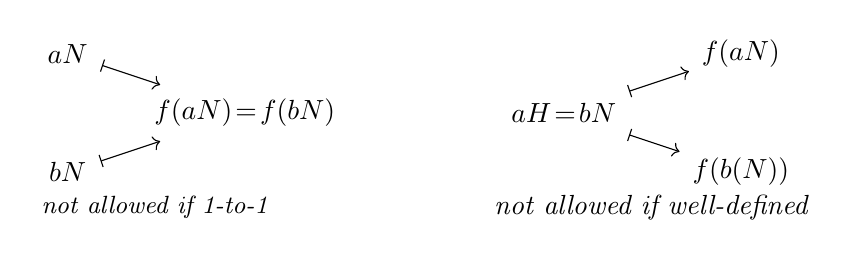
\begin{tikzpicture}[scale=.6,xscale=1.5]
    \begin{scope}[scale=2.5,inner sep=5pt]
      \node at (.5,-.8) {\small \emph{not allowed if 1-to-1}};
      \node (a) at (0,.5) {$aN$};
      \node (f) at (1,0) {$f(aN)\!=\!f(bN)$};
      \node (b) at (0,-.5) {$bN$};
      \draw[|->] (a) to (f);
      \draw[|->] (b) to (f);
    \end{scope}
    %%
    \begin{scope}[shift={(7,0)},scale=2.5,inner sep=4.5pt]
      \node at (.5,-.8) {\emph{not allowed if well-defined}};
      \node (fA) at (1,.5) {$f(aN)$};
      \node (aH) at (0,0) {$aH\!=\!bN$};
      \node (fB) at (1,-.5) {$f(b(N))$};
      \draw[|->] (aH) to (fA);
      \draw[|->] (aH) to (fB);
    \end{scope}
  \end{tikzpicture}
  \]

  Let's revisit the proof of the FHT, and the map
  \[
  \iota\colon G/N\to H,\qquad \iota(aN)=\phi(a),\qquad
  \text{where\, $N=\Ker(\phi)$}.
  \]

  Showing $\iota$ is well-defined is done as follows:
  \[
  aN\!=\!bN\hspace{1mm}\Rightarrow\hspace{1mm}
  b^{-1}aN\!=\!N \hspace{1mm}\Rightarrow\hspace{1mm}
  b^{-1}a\in\!N \hspace{1mm}\Rightarrow\hspace{1mm}
  \phi(b^{-1}a)\!=\!1
  \hspace{1mm}\Rightarrow\hspace{1mm}
  \phi(a)\!=\!\phi(b) \hspace{1mm}\Rightarrow\hspace{1mm}
  \iota(aN)\!=\!\iota(bN).
  \]
  Reversing each $\Rightarrow$ shows $\iota$ is 1-to-1.
  
  
\end{frame}

%%====================================================================

\begin{frame}{How to show two groups are isomorphic}
  
  The standard way to show $G\cong H$ is to \Alert{construct an
    isomorphism} $\phi\colon G\to H$.
  
  \medskip\Pause
  
  When the domain is a quotient, there is another method, due to the FHT. 
  
  \smallskip\Pause
  
  \begin{alertblock}{Useful technique}
    Suppose we want to show that $G/N\cong H$. There are two
    approaches: \Pause
    \begin{enumerate}
    \item[(i)] Define a map $\phi\colon G/N\to H$ and prove that it is
      \Galert{well-defined}, a \Alert{homomorphism}, and a
      \Balert{bijection}. \Pause
    \item[(ii)] Define a map $\phi\colon G\to H$ and prove that it is a
      \Alert{homomorphism}, a \Balert{surjection} (onto), and
      that \Palert{$\Ker\phi=N$}. 
    \end{enumerate}
  \end{alertblock}
  
  \smallskip\Pause
  
  Usually, Method~(ii) is easier. Showing well-definedness and
  injectivity can be tricky.
  
  \medskip\Pause
  
  For example, Method~(ii) works quite well in showing the
  following: \smallskip\Pause
  %%
  \begin{itemize}
  \item $\Z/\<n\>\cong\Z_n$; \smallskip\Pause
  \item $\Q^*/\<-1\>\cong\Q^+$; \smallskip\Pause
  \item $AB/B\cong A/(A\cap B)\quad$  \smallskip\Pause
  \item $G/(A\cap B)\cong (G/A)\times(G/B)\quad$ (if $G=AB$).
  \end{itemize}
  
\end{frame}

%%====================================================================

\begin{frame}{A picture of the isomorphism 
    $\iota\colon\Z/\<12\>\longrightarrow\Z_{12}$} \vspace{-4mm}

  %%
  %% Commutative diagram of FHT: Z/12Z
  %%
  \begin{figure}[!ht]
    \begin{tikzpicture}[scale=.65,box/.style={anchor=south}]
      \begin{scope}[shift={(-5.5,6.5)},scale=1]
        \tikzstyle{every node}=[font=\tiny]
        \tikzstyle{v} = [circle, draw, fill=lightgray,inner sep=0pt, minimum size=3mm]
        \node (-4) at (-3.9,0) {$\Large\Alert{\mathbf{\cdots}}$};
        \node (-3) at (-3,0) [v] {$-\!3$};
        \node (-2) at (-2,0) [v] {$-\!2$};
        \node (-1) at (-1,0) [v] {$-\!1$};
        \node (0) at (0,0) [v] {$0$};
        \node (1) at (1,0) [v] {$1$};
        \node (2) at (2,0) [v] {$2$};
        \node (3) at (3,0) [v] {$3$};
        \node (4) at (3.9,0) {$\Large\Alert{\mathbf{\cdots}}$};
        \draw [r] (-4) to (-3);
        \draw [r] (-3) to (-2); \draw [r] (-2) to (-1);
        \draw [r] (-1) to (0); \draw [r] (0) to (1);
        \draw [r] (1) to (2); \draw [r] (2) to (3);
        \draw [r] (3) to (4);
        \node at (0,1) {\large $\Z$};
        \draw [-stealth'] (4.4,0) to node[above] {\normalsize $\phi=\iota\circ\pi$} (7.5,0);
        \draw [-stealth'] (-1,-1.5) to node[below left] {\normalsize $\pi$} (.5,-4.5);
      \end{scope}
      %%
      \begin{scope}[shift={(5.5,6.5)},scale=1.85]
        \tikzstyle{every node}=[font=\scriptsize]
        \tikzstyle{v} = [circle, draw, fill=lightgray,inner sep=0pt, minimum size=3mm]
        \tikzstyle{r} = [draw,very thick,eRed,-stealth,bend right=8]
        \node (0) at (0:1) [v] {$0$};
        \node (1) at (30:1) [v] {$1$};
        \node (2) at (60:1) [v] {$2$};
        \node (3) at (90:1) [v] {$3$};
        \node (4) at (120:1) [v] {$4$};
        \node (5) at (150:1) [v] {$5$};
        \node (6) at (180:1) [v] {$6$};
        \node (7) at (210:1) [v] {$7$};
        \node (8) at (240:1) [v] {$8$};
        \node (9) at (270:1) [v] {$9$};
        \node (10) at (300:1) [v] {$10$};
        \node (11) at (330:1) [v] {$11$};
        \draw [r] (0) to (1); \draw [r] (1) to (2);
        \draw [r] (2) to (3); \draw [r] (3) to (4);
        \draw [r] (4) to (5); \draw [r] (5) to (6);
        \draw [r] (6) to (7); \draw [r] (7) to (8);
        \draw [r] (8) to (9); \draw [r] (9) to (10);
        \draw [r] (10) to (11); \draw [r] (11) to (0); 
        \node at (0,0) {\large $\Z_{12}$};
      \end{scope}
      %%
      \begin{scope}[shift={(0,0)},scale=1.5]
        \tikzstyle{r} = [draw,very thick,eRed,-stealth,bend right=8]
        \tikzstyle{every node}=[font=\scriptsize]
        \draw[cosetBlue, fill=cosetBlue] (0:2.6) circle (.28);
        \draw[cosetBlue, fill=cosetBlue] (0:1.4) circle (.28);
        \draw[cosetBlue, fill=cosetBlue,rotate=0] (1.4,-.28) rectangle (2.6,.28);
        %%
        \draw[cosetBlue, fill=cosetBlue,rotate=30] (0:2.65) circle (.28);
        \draw[cosetBlue, fill=cosetBlue,rotate=30] (0:1.45) circle (.28);
        \draw[cosetBlue, fill=cosetBlue,rotate=30] (1.45,-.28) rectangle (2.65,.28);
        %%
        \draw[cosetBlue, fill=cosetBlue,rotate=60] (0:2.7) circle (.28);
        \draw[cosetBlue, fill=cosetBlue,rotate=60] (0:1.5) circle (.28);
        \draw[cosetBlue, fill=cosetBlue,rotate=60] (1.5,-.28) rectangle (2.7,.28);
        %%
        \draw[cosetBlue, fill=cosetBlue,rotate=90] (0:2.75) circle (.28);
        \draw[cosetBlue, fill=cosetBlue,rotate=90] (0:1.55) circle (.28);
        \draw[cosetBlue, fill=cosetBlue,rotate=90] (1.55,-.28) rectangle (2.75,.28);
        %%
        \draw[cosetBlue, fill=cosetBlue,rotate=120] (0:2.8) circle (.28);
        \draw[cosetBlue, fill=cosetBlue,rotate=120] (0:1.6) circle (.28);
        \draw[cosetBlue, fill=cosetBlue,rotate=120] (1.6,-.28) rectangle (2.8,.28);
        %%
        %%
        \draw[cosetBlue, fill=cosetBlue,rotate=150] (0:2.85) circle (.28);
        \draw[cosetBlue, fill=cosetBlue,rotate=150] (0:1.65) circle (.28);
        \draw[cosetBlue, fill=cosetBlue,rotate=150] (1.65,-.28) rectangle (2.85,.28);
        %%
        \draw[cosetBlue, fill=cosetBlue,rotate=180] (0:2.9) circle (.28);
        \draw[cosetBlue, fill=cosetBlue,rotate=180] (0:1.7) circle (.28);
        \draw[cosetBlue, fill=cosetBlue,rotate=180] (1.7,-.28) rectangle (2.9,.28);
        %%
        \draw[cosetBlue, fill=cosetBlue,rotate=210] (0:2.95) circle (.28);
        \draw[cosetBlue, fill=cosetBlue,rotate=210] (0:1.75) circle (.28);
        \draw[cosetBlue, fill=cosetBlue,rotate=210] (1.75,-.28) rectangle (2.95,.28);
        %%
        \draw[cosetBlue, fill=cosetBlue,rotate=240] (0:2.4) circle (.28);
        \draw[cosetBlue, fill=cosetBlue,rotate=240] (0:1.2) circle (.28);
        \draw[cosetBlue, fill=cosetBlue,rotate=240] (1.2,-.28) rectangle (2.4,.28);
        %%
        \draw[cosetBlue, fill=cosetBlue,rotate=270] (0:2.45) circle (.28);
        \draw[cosetBlue, fill=cosetBlue,rotate=270] (0:1.25) circle (.28);
        \draw[cosetBlue, fill=cosetBlue,rotate=270] (1.25,-.28) rectangle (2.45,.28);
        %%
        \draw[cosetBlue, fill=cosetBlue,rotate=300] (0:2.5) circle (.28);
        \draw[cosetBlue, fill=cosetBlue,rotate=300] (0:1.3) circle (.28);
        \draw[cosetBlue, fill=cosetBlue,rotate=300] (1.3,-.28) rectangle (2.5,.28);
        %%
        \draw[cosetBlue, fill=cosetBlue,rotate=330] (0:2.55) circle (.28);
        \draw[cosetBlue, fill=cosetBlue,rotate=330] (0:1.35) circle (.28);
        \draw[cosetBlue, fill=cosetBlue,rotate=330] (1.35,-.28) rectangle (2.55,.28);
        %%
        \node [rotate=-17] (-17) at (200:1.2) {$\large\Alert{\mathbf{\ddots}}$};
        \node (-16) at (240:1.2) [v] {$-\!16$};
        \node (-15) at (270:1.25) [v] {$-\!15$};
        \node (-14) at (300:1.3) [v] {$-\!14$};
        \node (-13) at (330:1.35) [v] {$-\!13$};
        \node (-12) at (0:1.4) [v] {$-\!12$};
        \node (-11) at (30:1.45) [v] {$-\!11$};
        \node (-10) at (60:1.5) [v] {$-\!10$};
        \node (-9) at (90:1.55) [v] {$-9$};
        \node (-8) at (120:1.6) [v] {$-8$};
        \node (-7) at (150:1.65) [v] {$-7$};
        \node (-6) at (180:1.7) [v] {$-6$};
        \node (-5) at (210:1.75) [v] {$-5$};
        \node (-4) at (240:1.8) [v] {$-4$};
        \node (-3) at (270:1.85) [v] {$-3$};
        \node (-2) at (300:1.9) [v] {$-2$};
        \node (-1) at (330:1.95) [v] {$-1$};      
        \node (0) at (0:2) [v] {$0$};
        \node (1) at (30:2.05) [v] {$1$};
        \node (2) at (60:2.1) [v] {$2$};
        \node (3) at (90:2.15) [v] {$3$};
        \node (4) at (120:2.2) [v] {$4$};
        \node (5) at (150:2.25) [v] {$5$};
        \node (6) at (180:2.3) [v] {$6$};
        \node (7) at (210:2.35) [v] {$7$};
        \node (8) at (240:2.4) [v] {$8$};
        \node (9) at (270:2.45) [v] {$9$};
        \node (10) at (300:2.5) [v] {$10$};
        \node (11) at (330:2.55) [v] {$11$};
        \node (12) at (0:2.6) [v] {$12$};
        \node (13) at (30:2.65) [v] {$13$};
        \node (14) at (60:2.7) [v] {$14$};
        \node (15) at (90:2.75) [v] {$15$};
        \node (16) at (120:2.8) [v] {$16$};
        \node (17) at (150:2.85) [v] {$17$};
        \node (18) at (180:2.9) [v] {$18$};
        \node (19) at (210:2.95) [v] {$19$};
        \node [rotate=-15]  (20) at (230:3.02) {$\Large\Alert{\mathbf{\ddots}}$};
        %%
        \draw [r] (-17) to (-16);
        \draw [r] (-16) to (-15); \draw [r] (-15) to (-14);
        \draw [r] (-14) to (-13); \draw [r] (-13) to (-12);
        \draw [r] (-12) to (-11); \draw [r] (-11) to (-10);
        \draw [r] (-10) to (-9); \draw [r] (-9) to (-8);
        \draw [r] (-8) to (-7); \draw [r] (-7) to (-6);
        \draw [r] (-6) to (-5); \draw [r] (-5) to (-4);
        \draw [r] (-4) to (-3); \draw [r] (-3) to (-2);
        \draw [r] (-2) to (-1); \draw [r] (-1) to (0);
        \draw [r] (0) to (1); \draw [r] (1) to (2);
        \draw [r] (2) to (3); \draw [r] (3) to (4);
        \draw [r] (4) to (5); \draw [r] (5) to (6);
        \draw [r] (6) to (7); \draw [r] (7) to (8);
        \draw [r] (8) to (9); \draw [r] (9) to (10);
        \draw [r] (10) to (11); \draw [r] (11) to (12); 
        \draw [r] (12) to (13); \draw [r] (13) to (14);
        \draw [r] (14) to (15); \draw [r] (15) to (16);
        \draw [r] (16) to (17); \draw [r] (17) to (18);
        \draw [r] (18) to (19); \draw [r] (19) to (20);
        \node at (0,0) {\large $\Z/\<12\>$};
        \draw [-stealth'] (3,1) to [bend left=0] node[below right] {\normalsize $\iota$} (4,2.5);
      \end{scope}
    \end{tikzpicture}
  \end{figure}
  
\end{frame}

%%====================================================================
\section{The Isomorphism Theorems!}

%%====================================================================

\begin{frame}{The Isomorphism Theorems}
  
  The fundamental homomorphism theorem (FHT), or Noether's isomorphism theorem, is the first of four
  basic theorems about homomorphisms and their structure. 
  
  \bigskip\Pause
  
  These are commonly called ``\Alert{The Isomorphism
    Theorems}.''   \smallskip\Pause
  
  \begin{itemize}
  \item \Balert{Fundamental homomorphism
    theorem}: ``\emph{All homomorphic images are quotients}''  \smallskip\Pause
  \item \Balert{Correspondence theorem} or \Balert{lattice theorem}: Characterizes ``\emph{subgroups of quotients}'' \smallskip\Pause
  \item \Balert{Fraction theorem}: Characterizes ``\emph{quotients of quotients}'' \smallskip\Pause
  \item \Balert{Diamond theorem}: ``\emph{Duality of subquotients}.'' \smallskip\Pause
  \end{itemize}
  
  These all have analogues for other algebraic structures, e.g.,
  rings, vector spaces, modules, Lie algebras.
  
  \bigskip\Pause
  
  All of these theorems can look messy and unmotivated algebraically.
  
  \bigskip\Pause
  
  However, they all have beautiful visual interpretations, especially
  involving subgroup lattices.

  \bigskip\Pause

  For time reasons, we'll only really talk about the FHT and the lattice theorem.
  
\end{frame}

%%====================================================================

\begin{frame}{The correspondence theorem: subgroups of quotients}
  
  Given $N\normaleq G$, the quotient $G/N$ has a group structure, via
  $aN\cdot bN=abN$. \medskip\Pause
  
  Moreover, by the FHT, \emph{every} homomorphism image is a
  quotient. \smallskip\Pause
  
  \begin{exampleblock}{Natural question}
    What are the subgroups of a quotient?
  \end{exampleblock}
  
  \smallskip\Pause
  
  Fortunately, this has a simple answer that is easy to remember.
  
  \smallskip\Pause
  
  \begin{alertblock}{Correspondence theorem (informal)}
    The \Balert{subgroups of the quotient} $G/N$ are \Balert{quotients of the
      subgroups} $H\leq G$ that contain $N$. \medskip\Pause
    
    Moreover, ``most properties'' of $H/N\leq G/N$ are inherited from $H\leq G$.
  \end{alertblock}
  
  \smallskip\Pause
  
  This is best understood by interpreting the subgroup lattices of $G$
  and $G/N$.
  
  \medskip\Pause
  
  Let's do some examples for intuition, and then state the
  correspondence theorem formally.
  
\end{frame}

%%====================================================================

\begin{frame}{The correspondence theorem: subgroups of quotients}
  
  Compare $G=C_3 \rtimes C_4$ with the quotient by $N=\<r^3\>$. (This is HW 7.7.)
  %%
  %% Quotient Dic_6 / <r^3>  (Cayley diagrams)
  %%
  \[
  \begin{tikzpicture}[scale=.7,baseline=1.3ex,auto]
    \tikzstyle{every node}=[font=\footnotesize]
    \node at (2.5,1.95) {\normalsize $G/N$};
    \begin{scope}[shift={(.2,0)},scale=1]
      \draw (0,0) rectangle (1,.5);
      \node[anchor=south] at (.22,0) {$s$};
      \draw[anchor=south] (.73,0) node{$r^3\!s$};
      \node (123-b) at (1,.25) {};
      \node (123-out) at (.55,0) {}; \node (123-in) at (.55,.5) {};
    \end{scope}
    %%
    \begin{scope}[shift={(-1,-.9)}]  % was (-1.25,-.722)
      \draw (0,0) rectangle (1,.5);
      \node[anchor=south] at (.24,0) {$r^2s$};
      \draw[anchor=south] (.75,0) node{$r^5\!s$};
      \node (231-b) at (.2,0) {};
      \node (231-in) at (1,.25) {}; \node (231-out) at (0,.5) {};
    \end{scope}
    %%
    \begin{scope}[shift={(-1,.9)}]
      \draw (0,0) rectangle (1,.5);
      \node[anchor=south] at (.25,0) {$rs$};
      \draw[anchor=south] (.75,0) node{$r^4\!s$};
      \node (312-b) at (.2,.5) {};
      \node (312-in) at (0,0) {}; \node (312-out) at (1,.25) {};
    \end{scope}
    %%
    \begin{scope}[shift={(2,0)}]
      \draw (0,0) rectangle (1,.5);
      \node[anchor=south] at (.25,0) {$1$};
      \draw[anchor=south] (.75,0) node{$r^3$};
      \node (132-b) at (0,.25) {};
      \node (132-in) at (0,0) {}; \node (132-out) at (0,.5) {};
    \end{scope}
    %%
    \begin{scope}[shift={(-2.25,-2.15)}]
      \draw (0,0) rectangle (1,.5);
      \node[anchor=south] at (.25,0) {$r^2$};
      \draw[anchor=south] (.75,0) node{$r^5$};
      \node (213-b) at (.8,.5) {};
      \node (213-in) at (.3,.5) {}; \node (213-out) at (1,.25) {};
    \end{scope}
    %%
    \begin{scope}[shift={(-2.25,2.15)}]
      \draw (0,0) rectangle (1,.5);
      \node[anchor=south] at (.25,0) {$r$};
      \draw[anchor=south] (.75,0) node{$r^4$};
      \node (321-b) at (.8,0) {};
      \node (321-in) at (1,.25) {}; \node (321-out) at (.3,0) {};
    \end{scope}
    %%
    \begin{scope}[shift={(0,0)},shorten >= -2pt, shorten <= -2pt]
      \draw [bb] (123-b) -- (132-b); % node[midway,above]{$\;\;\;\;f$};
      \draw [bb] (231-b) -- (213-b); % node[midway,above]{$f$};
      \draw [bb] (312-b) -- (321-b); % 
      \draw [r] (123-out) to[bend left=24] (231-in); % %% [s]-->[sr]
      \draw [r] (231-out) to[bend left=35] (312-in); 
      \draw [r] (312-out) to[bend left=24] (123-in); % %% [1]-->[r]
      \draw [r] (132-out) to[bend right=35] (321-in); % %% [r]-->[r^2]
      \draw [r] (321-out) to[bend right=30] (213-in); % node[midway,above]{$r$};
      \draw [r] (213-out) to[bend right=35] (132-in); % node[midway,above]{$\;\;r$};
    \end{scope}
    %%
    %% Cayley graph 
    \begin{scope}[shift={(-8,.2)},scale=1.1]
      %%
      \tikzstyle{R-out} = [draw, very thick, eRed,-stealth,bend right=15]
      \tikzstyle{R-in} = [draw, very thick, eRed,-stealth,bend left=12]
      \tikzstyle{B} = [draw, very thick, eBlue,-stealth,bend left=25]
      \tikzstyle{every node}=[font=\small]
      %%
      \node at (-2.75,1.5) {\normalsize $G=C_3 \rtimes C_4$};
      \node (1) at (0:2) [v] {$1$};
      \node (r) at (60:2) [v] {$r$};
      \node (r2) at (120:2) [v] {$r^2$};
      \node (r3) at (180:2) [v] {$r^3$};
      \node (r4) at (240:2) [v] {$r^4$};
      \node (r5) at (300:2) [v] {$r^5$};
      \node (s) at (0:1) [v] {$s$};
      \node (rs) at (60:1) [v] {$rs$};
      \node (r2s) at (120:1) [v] {$r^2\!s$};
      \node (r3s) at (180:1) [v] {$r^3\!s$};
      \node (r4s) at (240:1) [v] {$r^4\!s$};
      \node (r5s) at (300:1) [v] {$r^5\!s$};
      \path[R-out] (1) to (r);
      \path[R-out] (r) to (r2);
      \path[R-out] (r2) to (r3);
      \path[R-out] (r3) to (r4);
      \path[R-out] (r4) to (r5);
      \path[R-out] (r5) to (1);
      \path[R-in] (rs) to (s);
      \path[R-in] (r2s) to (rs);
      \path[R-in] (r3s) to (r2s);
      \path[R-in] (r4s) to (r3s);
      \path[R-in] (r5s) to (r4s);
      \path[R-in] (s) to (r5s);
      %%
      \path[b] (1) to (s);
      \path[B] (s) to (r3);
      \path[b] (r3) to (r3s);
      \path[B] (r3s) to (1);
      %%
      \path[b] (r) to (rs);
      \path[B] (rs) to (r4);
      \path[b] (r4) to (r4s);
      \path[B] (r4s) to (r);
      %%
      \path[b] (r2) to (r2s);
      \path[B] (r2s) to (r5);
      \path[b] (r5) to (r5s);
      \path[B] (r5s) to (r2);
    \end{scope}
  \end{tikzpicture}
  \]  
  We know the subgroups structure of
  $G/N=\big\{N,\;rN,\;r^2N,\;sN,\;rsN,\;r^2\!sN\big\}\cong D_3$. \medskip\Pause
  
  ``\emph{The subgroups of the
    quotient $G/N$ are the quotients of the subgroups that contain $N$}.''
  
  %\vspace{2mm}

  %%
  %% Quotient Dic_6 / <r^3>  (shoeboxes)
  %%
  \[
  \begin{tikzpicture}[scale=.61]
    \tikzstyle{every node}=[font=\footnotesize,anchor=south]
    \begin{scope}[shift={(11,0)}]
    \node at (2,2.7) {``\emph{shoeboxes; lids on}''};
      \draw[thin,fill=faded] (0,0) rectangle (2,2.4);
      \draw[thin] (2,2.4) to (4,2.4); 
      \draw[thin] (0,1.6) to (4,1.6);
      \draw[thin] (0,.8) to (4,.8);
      \draw[thin] (2,0) to (4,0);
      \draw[thin] (4,0) to (4,2.4);
      \node at (1,.13) {$N$};
      \node at (3,.13) {$sN$};
      \node at (1,.93) {$rN$};
      \node at (3,.93) {$rsN$};
      \node at (1,1.73) {$r^2N$};
      \node at (3,1.73) {$r^2\!sN$};
      \node at (2,-.8) {\small $\<rN\>\leq G/N$};
    \end{scope}
    %%
    \begin{scope}[shift={(5.5,0)}]
      \draw[thin,fill=faded] (0,0) rectangle (2,2.4);
      \node at (2,2.7) {``\emph{shoeboxes; lids off}''};
      \draw[thin] (2,2.4) to (4,2.4); 
      \draw[thin] (0,1.6) to (4,1.6);
      \draw[thin] (0,.8) to (4,.8);
      \draw[thin] (2,0) to (4,0);
      \draw[thin] (4,0) to (4,2.4);
      \node at (.5,.13) {$1$};
      \node at (1.5,.13) {$r^3$};
      \node at (2.5,.13) {$s$};
      \node at (3.5,.13) {$r^3\!s$};
      \node at (.5,.93) {$r$};
      \node at (1.5,.93) {$r^4$};
      \node at (2.5,.93) {$rs$};
      \node at (3.5,.93) {$r^4\!s$};
      \node at (.5,1.73) {$r^2$};
      \node at (1.5,1.73) {$r^5$};
      \node at (2.5,1.73) {$r^2\!s$};
      \node at (3.5,1.73) {$r^5\!s$};
      \node at (2,-.8) {\small $\<r\>/N\leq G/N$};
    \end{scope}
    %%
    \begin{scope}[shift={(0,0)}]
      \draw[thin,fill=faded] (0,0) rectangle (2,2.4);
      \node at (2,2.7) {``\emph{shoes out of the box}''};
      \draw[thin] (2,2.4) to (4,2.4); 
      \draw[thin] (2,0) to (4,0);
      \draw[thin] (4,0) to (4,2.4);
      \node at (.5,.13) {$1$};
      \node at (1.5,.13) {$r^3$};
      \node at (2.5,.13) {$s$};
      \node at (3.5,.13) {$r^3\!s$};
      \node at (.5,.93) {$r$};
      \node at (1.5,.93) {$r^4$};
      \node at (2.5,.93) {$rs$};
      \node at (3.5,.93) {$r^4\!s$};
      \node at (.5,1.73) {$r^2$};
      \node at (1.5,1.73) {$r^5$};
      \node at (2.5,1.73) {$r^2\!s$};
      \node at (3.5,1.73) {$r^5\!s$};
      \node at (2,-.8) {\small $\<r\>\leq G$};
    \end{scope}
  \end{tikzpicture}
  \]
  
\end{frame}

%%====================================================================

\begin{frame}{The correspondence theorem: subgroups of quotients} \smallskip
  
  Here is the subgroup lattice of $G=C_3 \rtimes C_4$, and of the quotient
  $G/N$, where $N=\<r^3\>$.
  %%
  %% Quotient Dic_6 / <r^3>  (subgroup lattices)
  %%
  \[
  \begin{tikzpicture}[scale=.6,auto]
    \begin{scope}[shift={(0,-0)},shorten >= -2pt, shorten <= -2pt]
      \tikzstyle{every node}=[font=\small]
      \node(G) at (0,6) {$\<r,s\>$};
      \node(b) at (-1.5,4.5) {$\<r\>$};
      \node(aa) at (0,1.5) {$\<r^3\>$};
      \node(bb) at (-2,2.25) {\color{faded}$\<r^2\>$};
      \node(a) at (.5,24/7) {$\<s\>$};
      \node(ab) at (1.75,24/7) { $\<rs\>$};
      \node(ba) at (3,24/7) {$\<r^2\!s\>$};
      \node(1) at (0,0) {\color{faded}$\<1\>$};
      \draw[faded](1)--(aa); \draw[faded](1)--(bb);
      \draw(b)--(aa); \draw[faded](b)--(bb);
      \draw(G)--(a); \draw(G)--(ab); \draw(G)--(ba); \draw(G)--(b);
      \draw(aa)--(a); \draw(aa)--(ab); \draw(aa)--(ba);
    \end{scope}
    %%
    \begin{scope}[shift={(12.75,-0)},shorten >= -2pt, shorten <= -2pt]
      \tikzstyle{every node}=[font=\small]
      \node(G) at (0,6) {$\<rN,sN\>$};
      \node(b) at (-1.5,4.5) {$\<rN\>$};
      \node(aa) at (0,1.5) {$\<N\>$};
      \node(a) at (.5,24/7) {$\<sN\>$};
      \node(ab) at (1.75,24/7) { $\<rsN\>$};
      \node(ba) at (3,24/7) {$\<r^2\!sN\>$};
      \draw(b)--(aa);
      \draw(G)--(a); \draw(G)--(ab); \draw(G)--(ba); \draw(G)--(b);
      \draw(aa)--(a); \draw(aa)--(ab); \draw(aa)--(ba);
    \end{scope}
    %%
    \begin{scope}[shift={(6.25,-0)},shorten >= -2pt, shorten <= -2pt]
      \tikzstyle{every node}=[font=\footnotesize]
      \node(G) at (0,6.2) {$\<r,s\>/\<r^3\>$};
      \node(b) at (-1.5,4.5) {$\<r\>\!/\!\<r^3\>$};
      \node(aa) at (0,1.5) {$\<r^3\>\!/\!\<r^3\>$};
      \node(a) at (.4,24/7) {$\<s\>\!/\!\<r^3\>$};
      \node(ab) at (1.75,24/7) { $\<rs\>\!/\!\<r^3\>$};
      \node(ba) at (3.25,24/7) {$\<r^2s\>\!/\!\<r^3\>$};
      \draw(b)--(aa); 
      \draw(G)--(a); \draw(G)--(ab); \draw(G)--(ba); \draw(G)--(b);
      \draw(aa)--(a); \draw(aa)--(ab); \draw(aa)--(ba);
    \end{scope}
  \end{tikzpicture}
  \]
  ``\emph{The subgroups of the
    quotient $G/N$ are the quotients of the subgroups that contain $N$}.''
    
  \medskip

  %%
  %% Quotient Dic_6 / <r^3>  (shoeboxes)
  %%
  \[
  \begin{tikzpicture}[scale=.61]
    \tikzstyle{every node}=[font=\footnotesize,anchor=south]
    %%
    \begin{scope}[shift={(11,0)}]
      \node at (2,2.7) {``\emph{shoeboxes; lids on}''};
      \draw[thin,fill=faded] (0,0) rectangle (4,.8);
      \draw[thin] (0,2.4) to (4,2.4); 
      \draw[thin] (0,1.6) to (4,1.6);
      \draw[thin] (0,.8) to (4,.8);
      \draw[thin] (2,0) to (4,0);
      \draw[thin] (4,0) to (4,2.4);
      \draw[thin] (0,.8) to (0,2.4);
      \draw[thin] (2,0) to (2,2.4);
      \node at (1,.13) {$N$};
      \node at (3,.13) {$sN$};
      \node at (1,.93) {$rN$};
      \node at (3,.93) {$rsN$};
      \node at (1,1.73) {$r^2N$};
      \node at (3,1.73) {$r^2\!sN$};
      \node at (2,-.8) {\small $\<sN\>\leq G/N$};
    \end{scope}
    %%
    \begin{scope}[shift={(5.5,0)}]
      \node at (2,2.7) {``\emph{shoeboxes; lids off}''};
      \draw[thin,fill=faded] (0,0) rectangle (4,.8);
      \draw[thin] (0,2.4) to (4,2.4); 
      \draw[thin] (0,1.6) to (4,1.6);
      \draw[thin] (0,.8) to (4,.8);
      \draw[thin] (2,0) to (4,0);
      \draw[thin] (4,0) to (4,2.4);
      \draw[thin] (0,.8) to (0,2.4);
      \node at (.5,.13) {$1$};
      \node at (1.5,.13) {$r^3$};
      \node at (2.5,.13) {$s$};
      \node at (3.5,.13) {$r^3\!s$};
      \node at (.5,.93) {$r$};
      \node at (1.5,.93) {$r^4$};
      \node at (2.5,.93) {$rs$};
      \node at (3.5,.93) {$r^4\!s$};
      \node at (.5,1.73) {$r^2$};
      \node at (1.5,1.73) {$r^5$};
      \node at (2.5,1.73) {$r^2\!s$};
      \node at (3.5,1.73) {$r^5\!s$};
      \node at (2,-.8) {\small $\<s\>/N\leq G/N$};
      \draw[thin] (2,0) to (2,2.4);
    \end{scope}
    %%
    \begin{scope}[shift={(0,0)}]
      \node at (2,2.7) {``\emph{shoes out of the box}''};
      \draw[thin,fill=faded] (0,0) rectangle (4,.8);
      \draw[thin] (0,2.4) to (4,2.4); 
      \draw[thin] (0,.8) to (4,.8);
      \draw[thin] (2,0) to (4,0);
      \draw[thin] (4,0) to (4,2.4);
      \draw[thin] (0,.8) to (0,2.4);
      \node at (.5,.13) {$1$};
      \node at (1.5,.13) {$r^3$};
      \node at (2.5,.13) {$s$};
      \node at (3.5,.13) {$r^3\!s$};
      \node at (.5,.93) {$r$};
      \node at (1.5,.93) {$r^4$};
      \node at (2.5,.93) {$rs$};
      \node at (3.5,.93) {$r^4\!s$};
      \node at (.5,1.73) {$r^2$};
      \node at (1.5,1.73) {$r^5$};
      \node at (2.5,1.73) {$r^2\!s$};
      \node at (3.5,1.73) {$r^5\!s$};
      \node at (2,-.8) {\small $\<s\>\leq G$};
    \end{scope}
  \end{tikzpicture}
  \]

  \end{frame}

%%====================================================================

\begin{frame}{The correspondence theorem: subgroups of quotients} %\Pause

  \begin{alertblock}{Correspondence theorem (informally)}
    There is a bijection between \Alert{subgroups of $G/N$} and
    {\color{blue}subgroups of $G$ that contain $N$}. \medskip\Pause
    
    ``Everything that we want to be true'' about the subgroup lattice of $G/N$ 
    is inherited from the subgroup lattice of $G$. \medskip\Pause
    
    Most of these can be summarized as: 
    \[
    \text{``\emph{The \underline{\hspace{15mm}} of the quotient is
        just the quotient of the \underline{\hspace{15mm}}}''}
    \]
  \end{alertblock}
  
  \begin{block}{Correspondence theorem (formally)}
    Let $N\leq H\leq G$ and $N\leq K\leq G$ be chains of subgroups and
    $N\normaleq G$. Then
    %%
    \begin{enumerate}
    \item Subgroups of the quotient $G/N$ are quotients of the
      subgroup $H\leq G$ that contain $N$.
    \item $H/N\normaleq G/N$ if and only if $H\normaleq G$
    \item $[G/N:H/N]=[G:H]$
    \item $H/N\cap K/N=(H\cap K)/N$
    \item $\<H/N,K/N\>=\<H,K\>/N$
    \item $H/N$ is conjugate to $K/N$ in $G/N$ iff $H$ is
      conjugate to $K$ in $G$.
    \end{enumerate}
  \end{block}
  
\end{frame}

%%====================================================================

\begin{frame}{The correspondence theorem: subgroups of quotients} 
  
  All parts of the correspondence theorem have nice subgroup lattice
  interpretations. \medskip\Pause
  
  We've already interpreted the the first part. \medskip\Pause
  
  Here's what the next four parts say.

  %%
  %% Correspondence thoerem, parts 1-4.
  %%
  \[
  \begin{tikzpicture}[scale=.6]
    \begin{scope}[shift={(0,0)},scale=1.7]
      \node (G) at (0,4) {$G$};
      \node (H) at (0,3) {$H$};
      \node (K) at (0,2) {$K$};
      \node (N) at (0,1) {$N$};
      \node (1) at (0,0) {$1$};
      \draw[dashed] (H) circle [x radius=.3cm, y radius=.2cm];
      \draw (G) -- (H) node[left,pos=.5] {\footnotesize $a$}; 
      \draw (H) -- (K) node[left,pos=.5] {\footnotesize $b$};
      \draw (K) -- (N) node[left,pos=.5] {\footnotesize $c$};  
      \draw (N) to (1);
    \end{scope}
    %%
    \begin{scope}[shift={(3,0)},scale=1.7,shorten >= -2pt, shorten <= -2pt]
      \node (G/N) at (0,4) {$G/N$};
      \node (H/N) at (0,3) {$H/N$};
      \node (K/N) at (0,2) {$K/N$};
      \node (N/N) at (0,1) {$N/N$};
      \draw[dashed] (H/N) circle [x radius=.35cm, y radius=.25cm];
      \draw (G/N) -- (H/N) node[left,pos=.5] {\footnotesize $a$}; 
      \draw (H/N) -- (K/N) node[left,pos=.5] {\footnotesize $b$};
      \draw (K/N) -- (N/N) node[left,pos=.5] {\footnotesize $c$}; 
    \end{scope}
    %%%
    \begin{scope}[shift={(7,0)},scale=1.7]
      \node (G) at (0,4) {$G$};
      \node (HcupK) at (0,3) {$\<H,K\>$};
      \node (H) at (-.75,2.15) {$H$};
      \node (K) at (.75,1.85) {$K$};
      \node (HcapK) at (0,1) {$H\cap K$};
      \node (N) at (0,0) {$N$};
      \node (1) at (0,-1) {$1$};
      \draw (G) -- (HcupK);
      \draw (HcupK) -- (H); \draw (HcupK) -- (K);
      \draw (HcapK) -- (H); \draw (HcapK) -- (K);
      \draw (HcapK) -- (N);
      \draw (N) -- (1);
    \end{scope}
    %%
    \begin{scope}[shift={(11,0)},scale=1.7]
      \node (G/N) at (0,4) {$G/N$};
      \node (HcupK/N) at (0,3) {$\<H,K\>/N$};
      \node (H/N) at (-.75,2.15) {$H/N$};
      \node (K/N) at (.75,1.85) {$K/N$};
      \node (HcapK/N) at (0,1) {$(H\cap K)/N$};
      \node (N/N) at (0,0) {$N/N$};
      \draw (G/N) -- (HcupK/N);
      \draw (HcupK/N) -- (H/N); \draw (HcupK/N) -- (K/N);
      \draw (HcapK/N) -- (H/N); \draw (HcapK/N) -- (K/N);
      \draw (HcapK/N) -- (N/N);
    \end{scope}
    %%
    \begin{scope}[shift={(15.5,0)},scale=1.7]
      \node (G/N) at (0,4) {$G/N$};
      \node (HcupK/N) at (0,3) {$\<H/N,K/N\>$};
      \node (H/N) at (-.75,2.15) {$H/N$};
      \node (K/N) at (.75,1.85) {$K/N$};
      \node (HcapK/N) at (0,1) {$H/N\cap K/N$};
      \node (N/N) at (0,0) {$N/N$};
      \draw (G/N) -- (HcupK/N);
      \draw (HcupK/N) -- (H/N); \draw (HcupK/N) -- (K/N);
      \draw (HcapK/N) -- (H/N); \draw (HcapK/N) -- (K/N);
      \draw (HcapK/N) -- (N/N);
    \end{scope}
  \end{tikzpicture}
  \]
  
\end{frame}

%%====================================================================

\begin{frame}{The correspondence theorem: subgroups of quotients} 
  
  The last part says that we can characterize the conjugacy classes of $G/N$
  from those of $G$.
  %%
  %% Correspondence thoerem, part 5
  %%
  \[
  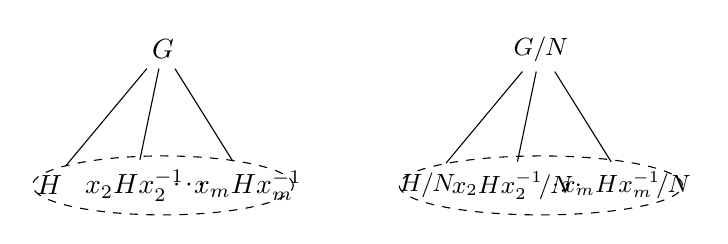
\begin{tikzpicture}[scale=.6]    
    \begin{scope}[shift={(0,0)},scale=1.2,yscale=.8]
      \tikzstyle{every node}=[font=\normalsize]
      \node (G) at (0,4) {$G$};
      \node (H) at (-2,1) {$H$};
      \node (H2) at (-.5,1) {$x_2Hx_2^{-1}$};
      \node (H3) at (.5,1) {$\cdots$};
      \node (Hl) at (1.5,1) {$x_m Hx_m^{-1}$};
      \draw (G)--(H); %node[above left,pos=.5] {\footnotesize $n$};
      \draw (G) -- (H2); \draw (G) -- (Hl);
      \draw[dashed] (0,1) circle [x radius=2.3cm, y radius=.65cm];
    \end{scope}
    %%
    \begin{scope}[shift={(8,0)},scale=1.2,yscale=.8]
      \tikzstyle{every node}=[font=\small]
      \node (G) at (0,4) {$G/N$};
      \node (H) at (-2,1) {$H/N$};
      \node (H2) at (-.5,1) {$x_2Hx_2^{-1}\!/N$};
      \node (H3) at (.5,1) {$\cdots$};
      \node (Hl) at (1.5,1) {$x_m Hx_m^{-1}\!/N$};
      \draw (G)--(H); %node[above left,pos=.5] {\footnotesize $n$};
      \draw (G) -- (H2); \draw (G) -- (Hl);
      \draw[dashed] (0,1) circle [x radius=2.5cm, y radius=.65cm];
    \end{scope}
  \end{tikzpicture}
  \]
  
  \medskip\Pause
  
  Let's apply that to find the conjugacy classes of $C_4\!\rtimes\!C_4$
  by inspection alone. Start by finding unicorns.
  %%
  %% Correspondence thoerem, part 5, C_4\rtimes C_4
  %%
  \[
  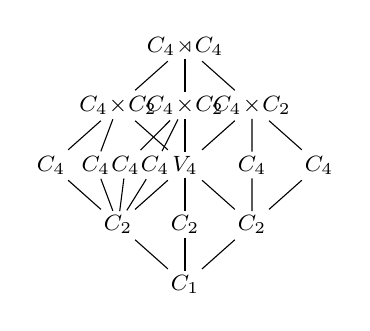
\begin{tikzpicture}[shorten >= -2pt, shorten <= -2pt,xscale=1.2,scale=.7]
    \tikzstyle{every node}=[font=\footnotesize]
    \begin{scope}[shift={(0,0)},scale=.75,yscale=1.6,scale=.9]
      \node (G) at (0,4) {$C_4\!\rtimes\!C_4$};
      \node (C4xC2-1) at (-1.5,3) {$C_4\!\times\!C_2$};
      \node (C4xC2-2) at (0,3) {$C_4\!\times\!C_2$};
      \node (C4xC2-3) at (1.5,3) {$C_4\!\times\!C_2$};
      \node (C4-1) at (-3,2) {$C_4$};
      \node (C4-2) at (-2,2) {$C_4$};
      \node (C4-3) at (-1.33,2) {$C_4$};
      \node (C4-4) at (-.67,2) {$C_4$};
      \node (C4-5) at (1.5,2) {$C_4$};
      \node (C4-6) at (3,2) {$C_4$};
      \node (V4) at (0,2) {$V_4$};
      \node (C2-1) at (-1.5,1) {$C_2$};
      \node (C2-2) at (0,1) {$C_2$};
      \node (C2-3) at (1.5,1) {$C_2$};
      \node (1) at (0,0) {$C_1$};
      \draw (G) to (C4xC2-1);
      \draw (G) to (C4xC2-2);
      \draw (G) to (C4xC2-3);
      \draw (C4xC2-1) to (C4-1);
      \draw (C4xC2-1) to (C4-2);
      \draw (C4xC2-1) to (V4); 
      \draw (C4xC2-2) to (C4-3);
      \draw (C4xC2-2) to (C4-4);
      \draw (C4xC2-2) to (V4); 
      \draw (C4xC2-3) to (C4-5);
      \draw (C4xC2-3) to (C4-6);
      \draw (C4xC2-3) to (V4);
      \draw (C4-1) to (C2-1); \draw (C4-2) to (C2-1);
      \draw (C4-3) to (C2-1); \draw (C4-4) to (C2-1);
      \draw (V4) to (C2-1); 
      \draw (V4) to (C2-2); \draw (V4) to (C2-3);
      \draw (C4-5) to (C2-3); \draw (C4-6) to (C2-3);
      \draw (C2-1) to (1); 
      \draw (C2-2) to (1); 
      \draw (C2-3) to (1);
    \end{scope}
  \end{tikzpicture}
  \]
  
\end{frame}

%%====================================================================

\begin{frame}{The correspondence theorem: subgroups of quotients} 
  
  The last part says that we can characterize the conjugacy classes of $G/N$
  from those of $G$.
  %%
  %% Correspondence thoerem, part 5
  %%
  \[
  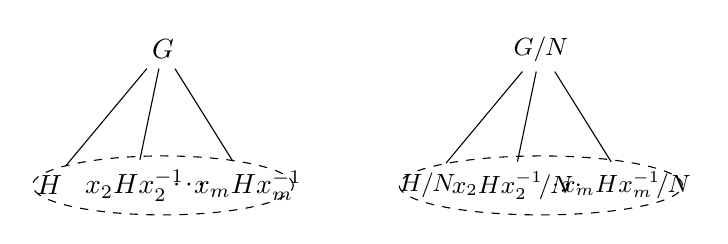
\begin{tikzpicture}[scale=.6]    
    \begin{scope}[shift={(0,0)},scale=1.2,yscale=.8]
      \tikzstyle{every node}=[font=\normalsize]
      \node (G) at (0,4) {$G$};
      \node (H) at (-2,1) {$H$};
      \node (H2) at (-.5,1) {$x_2Hx_2^{-1}$};
      \node (H3) at (.5,1) {$\cdots$};
      \node (Hl) at (1.5,1) {$x_m Hx_m^{-1}$};
      \draw (G)--(H); %node[above left,pos=.5] {\footnotesize $n$};
      \draw (G) -- (H2); \draw (G) -- (Hl);
      \draw[dashed] (0,1) circle [x radius=2.3cm, y radius=.65cm];
    \end{scope}
    %%
    \begin{scope}[shift={(8,0)},scale=1.2,yscale=.8]
      \tikzstyle{every node}=[font=\small]
      \node (G) at (0,4) {$G/N$};
      \node (H) at (-2,1) {$H/N$};
      \node (H2) at (-.5,1) {$x_2Hx_2^{-1}\!/N$};
      \node (H3) at (.5,1) {$\cdots$};
      \node (Hl) at (1.5,1) {$x_m Hx_m^{-1}\!/N$};
      \draw (G)--(H); %node[above left,pos=.5] {\footnotesize $n$};
      \draw (G) -- (H2); \draw (G) -- (Hl);
      \draw[dashed] (0,1) circle [x radius=2.5cm, y radius=.65cm];
    \end{scope}
  \end{tikzpicture}
  \]
  
  \medskip
  
  Let's apply that to find the conjugacy classes of $C_4\!\rtimes\!C_4$
  by inspection alone.
  %%
  %% Correspondence thoerem, part 5, C_4\rtimes C_4
  %%
  \[
  \begin{tikzpicture}[shorten >= -2pt, shorten <= -2pt,xscale=1.2,scale=.7]
    \tikzstyle{every node}=[font=\footnotesize]
    \begin{scope}[shift={(0,0)},scale=.75,yscale=1.6,scale=.9]
      \node (G) at (0,4) {$C_4\!\rtimes\!C_4$};
      \node (C4xC2-1) at (-1.5,3) {$C_4\!\times\!C_2$};
      \node (C4xC2-2) at (0,3) {$C_4\!\times\!C_2$};
      \node (C4xC2-3) at (1.5,3) {$C_4\!\times\!C_2$};
      \node (C4-1) at (-3,2) {$C_4$};
      \node (C4-2) at (-2,2) {$C_4$};
      \node (C4-3) at (-1.33,2) {$C_4$};
      \node (C4-4) at (-.67,2) {$C_4$};
      \node [faded] (C4-5) at (1.5,2) {$C_4$};
      \node [faded] (C4-6) at (3,2) {$C_4$};
      \node (V4) at (0,2) {$V_4$};
      \node (C2-1) at (-1.5,1) {$C_2$};
      \node [faded] (C2-2) at (0,1) {$C_2$};
      \node [faded] (C2-3) at (1.5,1) {$C_2$};
      \node [faded] (1) at (0,0) {$C_1$};
      \draw [thick] (G) to (C4xC2-1);
      \draw [thick] (G) to (C4xC2-2);
      \draw [thick] (G) to (C4xC2-3);
      \draw [thick] (C4xC2-1) to (C4-1);
      \draw [thick] (C4xC2-1) to (C4-2);
      \draw [thick] (C4xC2-1) to (V4); 
      \draw [thick] (C4xC2-2) to (C4-3);
      \draw [thick] (C4xC2-2) to (C4-4);
      \draw [thick] (C4xC2-2) to (V4); 
      \draw [faded] (C4xC2-3) to (C4-5);
      \draw [faded] (C4xC2-3) to (C4-6);
      \draw [thick] (C4xC2-3) to (V4);
      \draw [thick] (C4-1) to (C2-1); \draw [thick] (C4-2) to (C2-1);
      \draw [thick] (C4-3) to (C2-1); \draw [thick] (C4-4) to (C2-1);
      \draw [thick] (V4) to (C2-1); 
      \draw [faded] (V4) to (C2-2); \draw [faded] (V4) to (C2-3);
      \draw [faded] (C4-5) to (C2-3); \draw [faded] (C4-6) to (C2-3);
      \draw [faded] (C2-1) to (1); 
      \draw [faded] (C2-2) to (1); 
      \draw [faded] (C2-3) to (1);
    \end{scope}
    %%
    \begin{scope}[shift={(4.75,0)},scale=.75,yscale=1.6,scale=.9]
      \node (G) at (0,4) {$C_4\!\rtimes\!C_4$};
      \node (C4xC2-1) at (-1.5,3) {$C_4\!\times\!C_2$};
      \node (C4xC2-2) at (0,3) {$C_4\!\times\!C_2$};
      \node (C4xC2-3) at (1.5,3) {$C_4\!\times\!C_2$};
      \node [faded] (C4-1) at (-3,2) {$C_4$};
      \node [faded] (C4-2) at (-2,2) {$C_4$};
      \node [faded] (C4-3) at (-1.33,2) {$C_4$};
      \node [faded] (C4-4) at (-.67,2) {$C_4$};
      \node [faded] (C4-5) at (1.5,2) {$C_4$};
      \node [faded] (C4-6) at (3,2) {$C_4$};
      \node (V4) at (0,2) {$V_4$};
      \node [faded] (C2-1) at (-1.5,1) {$C_2$};
      \node (C2-2) at (0,1) {$C_2$};
      \node [faded] (C2-3) at (1.5,1) {$C_2$};
      \node [faded] (1) at (0,0) {$C_1$};
      \draw [thick] (G) to (C4xC2-1); \draw [thick] (G) to (C4xC2-2);
      \draw [thick] (G) to (C4xC2-3);
      \draw [faded] (C4xC2-1) to (C4-1);
      \draw [faded] (C4xC2-1) to (C4-2);
      \draw [thick] (C4xC2-1) to (V4);
      \draw [faded] (C4xC2-2) to (C4-3);
      \draw [faded] (C4xC2-2) to (C4-4);
      \draw [thick] (C4xC2-2) to (V4); 
      \draw [faded] (C4xC2-3) to (C4-5);
      \draw [faded] (C4xC2-3) to (C4-6);
      \draw [thick] (C4xC2-3) to (V4);
      \draw [faded] (C4-1) to (C2-1); \draw [faded] (C4-2) to (C2-1);
      \draw [faded] (C4-3) to (C2-1); \draw [faded] (C4-4) to (C2-1);
      \draw [faded] (V4) to (C2-1);
      \draw [thick] (V4) to (C2-2); 
      \draw [faded] (V4) to (C2-3);
      \draw [faded] (C4-5) to (C2-3); \draw [faded] (C4-6) to (C2-3);
      \draw [faded] (C2-1) to (1); \draw [faded] (C2-2) to (1); 
      \draw [faded] (C2-3) to (1);
    \end{scope}
    %%
    \begin{scope}[shift={(9.5,0)},scale=.75,yscale=1.6,scale=.9]
      \node (G) at (0,4) {$C_4\!\rtimes\!C_4$};
      \node (C4xC2-1) at (-1.5,3) {$C_4\!\times\!C_2$};
      \node (C4xC2-2) at (0,3) {$C_4\!\times\!C_2$};
      \node (C4xC2-3) at (1.5,3) {$C_4\!\times\!C_2$};
      \node [faded] (C4-1) at (-3,2) {$C_4$};
      \node [faded] (C4-2) at (-2,2) {$C_4$};
      \node [faded] (C4-3) at (-1.33,2) {$C_4$};
      \node [faded] (C4-4) at (-.67,2) {$C_4$};
      \node (C4-5) at (1.5,2) {$C_4$};
      \node (C4-6) at (3,2) {$C_4$};
      \node (V4) at (0,2) {$V_4$};
      \node [faded] (C2-1) at (-1.5,1) {$C_2$};
      \node [faded] (C2-2) at (0,1) {$C_2$};
      \node (C2-3) at (1.5,1) {$C_2$};
      \node [faded] (1) at (0,0) {$C_1$};
      \draw [thick] (G) to (C4xC2-1);
      \draw [thick] (G) to (C4xC2-2); \draw [thick] (G) to (C4xC2-3);
      \draw [faded] (C4xC2-1) to (C4-1);
      \draw [faded] (C4xC2-1) to (C4-2);
      \draw [thick] (C4xC2-1) to (V4);
      \draw [faded] (C4xC2-2) to (C4-3);
      \draw [faded] (C4xC2-2) to (C4-4);
      \draw [thick] (C4xC2-2) to (V4); 
      \draw [thick] (C4xC2-3) to (C4-5);
      \draw [thick] (C4xC2-3) to (C4-6);
      \draw [thick] (C4xC2-3) to (V4);
      \draw [faded] (C4-1) to (C2-1); \draw [faded] (C4-2) to (C2-1);
      \draw [faded] (C4-3) to (C2-1); \draw [faded] (C4-4) to (C2-1);
      \draw [faded] (V4) to (C2-1); \draw [faded] (V4) to (C2-2); 
      \draw [thick] (V4) to (C2-3);
      \draw [thick] (C4-5) to (C2-3); \draw [thick] (C4-6) to (C2-3);
      \draw [faded] (C2-1) to (1); \draw [faded] (C2-2) to (1); 
      \draw [faded] (C2-3) to (1);
    \end{scope}
  \end{tikzpicture}
  \]
  
\end{frame}

%%====================================================================

\begin{frame}{The correspondence theorem: subgroups of quotients} %\Pause
  
  Let's prove the first (main) part of the correspondence theorem.
  
  \begin{block}{Correspondence theorem (first part)}
    The subgroups of the quotient $G/N$ are quotients of the
    subgroup $H\leq G$ that contain $N$.
  \end{block}
  
  \begin{exampleblock}{Proof} \pause
    Let $S$ be a subgroup of $G/N$. \Pause Then $S$ is a collection of
    cosets, i.e.,
    \[
    S=\big\{hN\mid h\in H\big\},
    \]
    for some \Balert{subset} $H\subseteq G$. \Pause We just need to
    show that $H$ is a subgroup. \medskip\pause

    We'll use the \Balert{one-step subgroup test}: take
    $h_1N,\,h_2N\in S$. \Pause Then $S$ must also contain
    \begin{equation}\label{eqn:H/N}
    (h_1N)(h_2N)^{-1}=(h_1N)(h_2^{-1}N)=(h_1h_2^{-1})N.
    \end{equation}
    That is, $h_1h_2^{-1}\in H$, which means that $H$ is a
    subgroup. $\hfill\checkmark$ \medskip\pause

    Conversely, suppose that $N\leq H\leq G$. \Pause The one-step subgroup
    test shows that $H/N\leq G/N$; see Eq.~\eqref{eqn:H/N}. $\hfill\Box$
  \end{exampleblock}
  
  \smallskip\Pause
  
  The other parts are straightforward and will be left as exercises.
\end{frame}

%%====================================================================
\section{Another fun group to play with!}

%%====================================================================

\begin{frame}{Groups of matrices} %\smallskip
  
  \Pause
  
  \begin{block}{Definition}
    Let $\Mat_n(\F)$ be the set of $n\times n$ matrices with
    \Balert{coefficients from $\F$}.
  \end{block}

  \smallskip \pause

  $\F$ is a ``field'' -- you can add, subtract, multiply, and divide, and everything commutes. \pause Examples of fields? \pause
  \begin{itemize}
    \item $\Q$, the rationals
    \item $\R$, the real numbers
    \item $\C$, the complex numbers
    \item Weirdly, $\Z_p$ for $p$ a prime (``finite fields'')
  \end{itemize} \pause

  \begin{alertblock}{Careful:}
    $\Mat_n(\F)$ is not a group under multiplication! \pause Why not?
  \end{alertblock}
  
  \begin{block}{Definition}
    Thqe \Alert{general linear group} of degree $n$ over $\F$ is the
    set of invertible matrices with coefficients from $\F$:
    \[
    \GL_n(\F)=\big\{A\in\Mat_n(\F)\mid \det A\neq 0\big\}. 
    \]
    \Pause The \Alert{special linear group} is the subgroup of matrices with
    determinant $1$:
    \[
    \SL_n(\F)=\big\{A\in\GL_n(\F)\mid\det A=1\big\}.
    \]
  \end{block}

\end{frame}

%%====================================================================

\begin{frame}{Groups of $2\times 2$ matrices over $\Z_3$} \pause

  \begin{exampleblock}{$\Mat_2(\Z_3)$}
    Give an example of:
    \begin{itemize}
      \item a $2\times 2$ matrix 
      \item whose elements are all in $\Z_3$.
    \end{itemize} 
    
  \end{exampleblock} \pause

  \begin{exampleblock}{$\GL_2(\Z_3)$ (or you might see $\GL(2, \Z_3)$)}
    Give an example of:
    \begin{itemize}
      \item a $2\times 2$ matrix 
      \item whose elements are all in $\Z_3$ \pause
      \item and whose determinant is nonzero.
    \end{itemize} 
  \end{exampleblock} \pause

  \begin{exampleblock}{$\SL_2(\Z_3)$ aka $\SL(2, \Z_3)$}
    Give an example of:
    \begin{itemize}
      \item a $2\times 2$ matrix 
      \item whose elements are all in $\Z_3$
      \item and whose determinant is nonzero \pause
      \item and whose determinant is specifically 1.
    \end{itemize} 
  \end{exampleblock}
  
\end{frame}

%%====================================================================

\begin{frame}{$\SL(2, \Z_3)$}
  How many matrices are there in $\SL(2, \Z_3)$? 

  \medskip \pause

  Here are two good ones to play with:
  \[
  A=\begin{bmatrix}2&1\\0&2\end{bmatrix}
  =\begin{bmatrix}-1&1\\0&-1\end{bmatrix},\qquad
  B=\begin{bmatrix}2&0\\1&2\end{bmatrix}
  =\begin{bmatrix}-1&0\\1&-1\end{bmatrix}. 
  \]
\end{frame}

%%====================================================================

\begin{frame}{The ``subgroup'' and ``quotient'' operations commute} 
  
  \begin{alertblock}{Key idea}
    The \Balert{quotient of a subgroup} is just the \Balert{subgroup
      of the quotient}.
  \end{alertblock}

  \medskip\Pause
  
  \textbf{Example}: Consider the group $G=\SL_2(\Z_3)$.
  %%
  %% Quotient of a subgroup of SL_2(Z_3)
  %%
  \[
  \hspace*{-2mm}
  \begin{tikzpicture}[node distance=1cm,shorten >= -2pt, shorten <= -2pt,scale=.6]
    %%
    \begin{scope}[shift={(0,0)}]
      \tikzstyle{every node}=[font=\footnotesize]
      \node (1) {$\<1\>$};
      \node (a3) at (-2.5,2) {$\<a^3\>$};
      \node (a2) at (.9,3) {$\<a^2\>$};
      \node (b2) at (2,3) {$\<b^2\>$};
      \node (abab) at (3.1,3) {$\<(ab)^2\>$};
      \node (baba) at (4.35,3) {$\<(ba)^2\>$};
      \node (a2b) at (-3.75,4) {$\<a^2b\>$};
      \node (aba) at (-2.5,4) {$\<aba\>$};
      \node (ab2) at (-1.25,4) {$\<ab^2\>$};
      \node (a) at (.5,5) {$\<a\>$};
      \node (b) at (1.6,5) {$\<b\>$};
      \node (ab) at (2.7,5) {$\<ab\>$};
      \node (ba) at (3.95,5) {$\<ba\>$};
      \node (a2b-ab2) at (-2.5,6) {$\<a^2b,ab^2\>$};
      \node (G) at (0,8) {$G=\<a,b\>$};
      \draw (1) -- (a3);
      \draw (1) -- (a2);
      \draw (1) -- (b2);
      \draw (1) -- (abab);
      \draw (1) -- (baba);
      \draw (a3) -- (a2b);
      \draw (a3) -- (aba);
      \draw (a3) -- (ab2);
      \draw (a3) -- (a);
      \draw (a3) -- (b);
      \draw (a3) -- (ab);
      \draw (a3) -- (ba);
      \draw (a2) -- (a);
      \draw (b2) -- (b);
      \draw (abab) -- (ab);
      \draw (baba) -- (ba);
      \draw (a2b) -- (a2b-ab2);
      \draw (aba) -- (a2b-ab2);
      \draw (ab2) -- (a2b-ab2);
      \draw (G) -- (a2b-ab2);
      \draw (G) -- (a);
      \draw (G) -- (b);
      \draw (G) -- (ab);
      \draw (G) -- (ba);
    \end{scope}
    %%
    \begin{scope}[shift={(10,0)}]
      \tikzstyle{every node}=[font=\footnotesize]
      \node (1) at (-2.5,0) {\color{faded}$\<1\>$};
      \node (a3) at (-2.5,2) {$\<a^3\>$};
      \node (a2b) at (-3.75,4) {$\<a^2b\>$};
      \node (aba) at (-2.5,4) {$\<aba\>$};
      \node (ab2) at (-1.25,4) {$\<ab^2\>$};
      \node (a2b-ab2) at (-2.5,6) {$\<a^2b,ab^2\>$};
      \draw[faded] (1) -- (a3);
      \draw (a3) -- (a2b);
      \draw (a3) -- (aba);
      \draw (a3) -- (ab2);
      \draw (a2b) -- (a2b-ab2);
      \draw (aba) -- (a2b-ab2);
      \draw (ab2) -- (a2b-ab2);
      \node at (-2.5,7.5) {\normalsize subgroup $\bm{H\cong Q_8}$};
    \end{scope}
    %%
    \begin{scope}[shift={(15,0)}]
      \tikzstyle{every node}=[font=\scriptsize]
      \node (a3) at (-2.5,2) {$\<a^3\>/N$};
      \node (a2b) at (-3.75,4) {\hspace{-2mm}$\<a^2b\>/N$};
      \node (aba) at (-2.5,4) {$\<aba\>/N$};
      \node (ab2) at (-1.25,4) {$\<ab^2\>/N$};
      \node (a2b-ab2) at (-2.5,6) {\hspace{2mm}$\<a^2b,ab^2\>/N$};
      \draw (a3) -- (a2b);
      \draw (a3) -- (aba);
      \draw (a3) -- (ab2);
      \draw (a2b) -- (a2b-ab2);
      \draw (aba) -- (a2b-ab2);
      \draw (ab2) -- (a2b-ab2);
      \node at (-2.5,7.5) {\normalsize $\bm{H/N\cong V_4}$};
      \node at (-2.5,1) {\normalsize ``\emph{quotient of the subgroup}''};
    \end{scope}
  \end{tikzpicture}
  \]
  
\end{frame}

%%====================================================================

\begin{frame}{The ``subgroup'' and ``quotient'' operations commute} 
  
  \begin{alertblock}{Key idea}
    The \Balert{quotient of a subgroup} is just the \Balert{subgroup
      of the quotient}.
  \end{alertblock}
  
  \medskip
  
  \textbf{Example}: Consider the group $G=\SL_2(\Z_3)$. %\vspace{-4mm}
  %%
  %% Subgroup of a quotient of SL_2(Z_3)
  %%
  \[
  \hspace*{-2mm}
  \begin{tikzpicture}[node distance=1cm,shorten >= -2pt, shorten <= -2pt,scale=.6]
    \begin{scope}[shift={(0,0)}]
      \tikzstyle{every node}=[font=\tiny]
      \node at (-3.5,7.5) {\normalsize quotient $\bm{G/N\cong A_4}$};
      \node (1) {\color{faded}$\<1\>$};
      \node (a3) at (-2.5,2) {$\<a^3\>/N$};
      \node (a2) at (.9,3) {\color{faded}$\<a^2\>$};
      \node (b2) at (2,3) {\color{faded}$\<b^2\>$};
      \node (abab) at (3.1,3) {\color{faded}$\<(ab)^2\>$};
      \node (baba) at (4.35,3) {\color{faded}$\<(ba)^2\>$};
      \node (a2b) at (-3.75,4) {$\<a^2b\>/N$};
      \node (aba) at (-2.5,4) {$\<aba\>/N$};
      \node (ab2) at (-1.25,4) {$\<ab^2\>/N$};
      \node (a) at (.5,5) {$\<a\>/N$};
      \node (b) at (1.6,5) {$\<b\>/N$};
      \node (ab) at (2.7,5) {$\<ab\>/N$};
      \node (ba) at (3.95,5) {$\<ba\>/N$};
      \node (a2b-ab2) at (-2.5,6) {$\<a^2b,ab^2\>/N$};
      \node (G) at (0,8) {$\<a,b\>/N$};
      \draw[faded] (1) -- (a3);
      \draw[faded] (1) -- (a2);
      \draw[faded] (1) -- (b2);
      \draw[faded] (1) -- (abab);
      \draw[faded] (1) -- (baba);
      \draw (a3) -- (a2b);
      \draw (a3) -- (aba);
      \draw (a3) -- (ab2);
      \draw (a3) -- (a);
      \draw (a3) -- (b);
      \draw (a3) -- (ab);
      \draw (a3) -- (ba);
      \draw[faded] (a2) -- (a);
      \draw[faded] (b2) -- (b);
      \draw[faded] (abab) -- (ab);
      \draw[faded] (baba) -- (ba);
      \draw (a2b) -- (a2b-ab2);
      \draw (aba) -- (a2b-ab2);
      \draw (ab2) -- (a2b-ab2);
      \draw (G) -- (a2b-ab2);
      \draw (G) -- (a);
      \draw (G) -- (b);
      \draw (G) -- (ab);
      \draw (G) -- (ba);
    \end{scope}
    %%
    \begin{scope}[shift={(11,0)}]
      \tikzstyle{every node}=[font=\tiny]
      \node at (-2.5,7.5) {\normalsize$\bm{V_4\cong H/N\leq G/N}$};
      \node (a3) at (-2.5,2) {$\<a^3\>/N$};
      \node (a2b) at (-3.75,4) {$\<a^2b\>/N$};
      \node (aba) at (-2.5,4) {$\<aba\>/N$};
      \node (ab2) at (-1.25,4) {$\<ab^2\>/N$};
      \node (a2b-ab2) at (-2.5,6) {$\<a^2b,ab^2\>/N$};
      \draw (a3) -- (a2b);
      \draw (a3) -- (aba);
      \draw (a3) -- (ab2);
      \draw (a2b) -- (a2b-ab2);
      \draw (aba) -- (a2b-ab2);
      \draw (ab2) -- (a2b-ab2);
      \node at (-2.5,1) {\normalsize ``\emph{subgroup of the quotient}''};
    \end{scope}
  \end{tikzpicture}
  \]
  
\end{frame}

%%====================================================================

\end{document}

%%====================================================================
